% CVPR 2025 Paper Template; see https://github.com/cvpr-org/author-kit

\documentclass[12pt,onecolumn,letterpaper]{article}

%%%%%%%%% PAPER TYPE  - PLEASE UPDATE FOR FINAL VERSION
% \usepackage{cvpr}              % To produce the CAMERA-READY version
\usepackage[review]{cvpr}      % To produce the REVIEW version
% \usepackage[pagenumbers]{cvpr} % To force page numbers, e.g. for an arXiv version

% Import additional packages in the preamble file, before hyperref
%
% --- inline annotations
%
\newcommand{\red}[1]{{\color{red}#1}}
\newcommand{\todo}[1]{{\color{red}#1}}
\newcommand{\TODO}[1]{\textbf{\color{red}[TODO: #1]}}
% --- disable by uncommenting  
% \renewcommand{\TODO}[1]{}
% \renewcommand{\todo}[1]{#1}



% It is strongly recommended to use hyperref, especially for the review version.
% hyperref with option pagebackref eases the reviewers' job.
% Please disable hyperref *only* if you encounter grave issues, 
% e.g. with the file validation for the camera-ready version.
%
% If you comment hyperref and then uncomment it, you should delete *.aux before re-running LaTeX.
% (Or just hit 'q' on the first LaTeX run, let it finish, and you should be clear).
\definecolor{cvprblue}{rgb}{0.21,0.49,0.74}
\usepackage[pagebackref,breaklinks,colorlinks,allcolors=cvprblue]{hyperref}

%%%%%%%%% PAPER ID  - PLEASE UPDATE
\def\paperID{17349}% *** Enter the Paper ID here
\def\confName{WPO NOFO}
\def\confYear{2025}

%%%%%%%%% TITLE - PLEASE UPDATE
\title{Verfication and Validation of SmokeViz: An Ensemble-Based Deep Learning Model for Identifying Wildfire Smoke Plumes in Satellite Imagery}

%%%%%%%%% AUTHORS - PLEASE UPDATE
\author{First Author\\
Institution1\\
Institution1 address\\
{\tt\small firstauthor@i1.org}
% For a paper whose authors are all at the same institution,
% omit the following lines up until the closing ``}''.
% Additional authors and addresses can be added with ``\and'',
% just like the second author.
% To save space, use either the email address or home page, not both
\and
Second Author\\
Institution2\\
First line of institution2 address\\
{\tt\small secondauthor@i2.org}
}

\begin{document}
\maketitle
%\begin{abstract}
    The global increase in the frequency and intensity of wildfires underscores the need for advancements in fire monitoring techniques. In order to investigate deep learning approaches for detecting and tracking wildfires and the related human health impacts, we present SmokeViz, a large scale machine learning dataset of smoke plumes in satellite imagery. To build the dataset, we refine a set of human-generated annotations created by analysts at the National Oceanic and Atmospheric Administration. Each annotation gives a general temporal and geographical approximation of smoke plumes but at variable and, primarily, low temporal resolution. We present an innovative solution for refining the temporal and spatial resolution in the given analyst annotations by leveraging the semi-supervised method, pseudo-labeling. Unlike typical pseudo-labeling applications that aim to increase the number of labeled samples, the objective is to use pseudo-labels to refine an existing but course-grained set of annotations. We train a deep learning model to generate pseudo-labels that pinpoint the singular, most representative, satellite image to match the smoke annotation within the given temporal range. By identifying the most representative imagery of smoke plumes for a given smoke annotation, the study seeks to create an accurate and relevant machine learning dataset. The resulting SmokeViz dataset is anticipated to be an instrumental tool in developing further machine learning models for studying wildfires and is publically availble at [aws download link].
\end{abstract}
    
\section{Problem Statement}
\label{sec:intro}

In part due to public policy, the average levels of fine particulate matter (PM\textsubscript{2.5}) in the US have generally been declining over the past few decades \cite{clean_air_act}. Despite those improvements, the contribution of wildfire smoke to PM\textsubscript{2.5} concentrations in the US has been calculated to have more than doubled between 2010 to 2020, accounting for up to half of the overall PM\textsubscript{2.5} exposure in Western regions \cite{smoke_PM}. Increases in PM\textsubscript{2.5} due to wildfire smoke are concerning since ambient PM\textsubscript{2.5} exposure is a leading environmental risk factor for adverse health effects and premature mortality \cite{smoke_mortality}.  These risks underscore the necessity for efficient and effective monitoring methods to mitigate the adverse health impacts associated with wildfire smoke. 

Satellite imagery, equipped with state-of-the-art sensors, such as the Advanced Baseline Imager (ABI) on the Geostationary Operational Environmental Satellites (GOES) \cite{goes}, have revolutionized environmental monitoring. Compared to orbiting satellites such as the Suomi or Sentinel satellites, geostationary satellites maintain constant observation over a fixed area. GOES offers the advantage being able to reliably and consistently capture the dynamic behavior of wildfire smoke plumes. In turn, GOES capabilities can provide critical insights into the concentration and movement of smoke particulates, facilitating real-time assessments of air quality.

Current fire detection algorithms rely primarily on calculating the fire radiative power (FRP) of active fires using near-infrared (NIR) satellite bands \cite{frp}. When fires have thick smoke plumes, the smoke can obfuscate a satellite's view of an active fire, making FRP impossible to calculate. If combined with FRP calculations, a real-time widlfire smoke plume analysis product can deliver additional insight into an active wildfire's activity level. 

Generally, integrating satellite imagery into wildfire smoke monitoring provides real-time data that can improve the timeliness of public health planning and response. By mapping the spread and density of smoke, health authorities can issue prompt warnings, implement evacuation protocols, and deploy resources effectively to mitigate health risks. Furthermore, long-term data gathered from satellite observations can aid in understanding the broader impacts of wildfire smoke on public health, influencing policy decisions and preventive measures. 

To address the need for a timely smoke analysis product, we present SmokeViz, an ensemble based deep learning method to identify and classify smoke plumes in satellite imagery. The model is a result of a successful project at the Global Systems Laboratory at the National Oceanic and Atmospheric Administration (NOAA) to build a large scale dataset of smoke plumes in GOES imagery. Keeping in mind the correlation between both the quality and quantity of data with deep learning model performance, we introduced the largest known smoke plume dataset, containing over 180,000 samples. The resulting dataset was used to train an ensemble of deep learning models that decorrelate errors by varying the inductive biases and give a more robust prediction than any singular model. 

We propose bringing SmokeViz to NOAA's Fire Weather Testbed to evaluate it's capabilities to (1) replace or enchance NOAA's current human annotated smoke product and (2) improve latency in NOAA's smoke dispersion models by using it as a smoke analysis product. The following subsections elaborate on the current needs for SmokeViz in these two application areas. 

\subsection{Replacing the Hazard Mapping Systems Smoke Product} 

\begin{figure*}
    \centering
    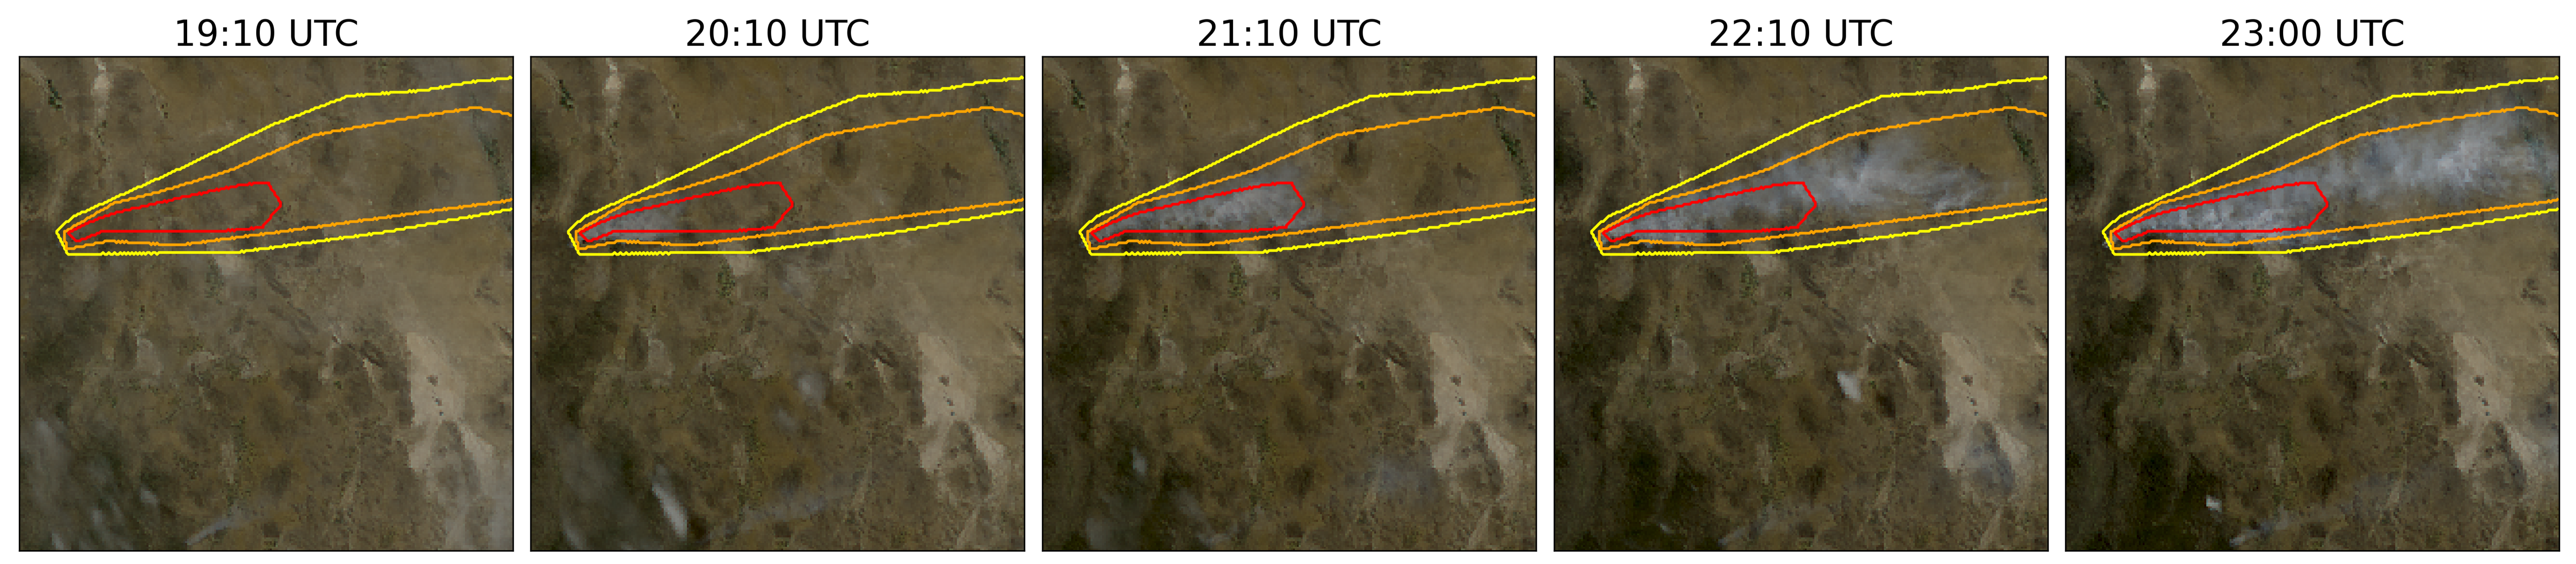
\includegraphics[width=\linewidth]{figures/TIMELAPSE_FINAL2.png}
    \caption{True color GOES-East imagery from May 5th, 2022, Southeast New Mexico (\(31.38^{\circ}\)N, \(107.87^{\circ}\)W) during the start of the Foster Fire. The red, orange and yellow lines represent the heavy, medium and low density HMS smoke annotations that span 19:10\textendash23:00 UTC.}
    \label{timelapse}
\end{figure*}

The National Oceanic and Atmospheric Administration (NOAA) manages environmental satlelite programs such as the Hazard Mapping System (HMS) program that uses an aggregation of satellite data to generate active fire and smoke data \cite{hms, hms_val}. The HMS smoke product \cite{hms, hms_val} is generated by human visual inspection of GOES satellite imagery for smoke identification. Trained satellite analysts use movement characteristics to help identify smoke by scanning through a time series of satellite images. When visual inspection indicates smoke, the analyst will draw a polygon that corresponds to the geolocation and density of smoke. HMS smoke analysis data gives the coordinates of the smoke perimeter as a polygon and classifies the smoke by density within a given time window. The time windows can range from instantaneous (same start/end time) to lengths of 22 hours, with an average time window around 3 hours. While the true bounds of the smoke can change within the larger time spans (figure \ref{timelapse}), the analyst is making an approximation that should reflect the smoke coverage over the duration of the time window. The density information is qualitatively determined by each analyst based on the apparent smoke opacity in the satellite imagery and categorized as either light, medium or heavy as seen in figure \ref{densities}a \cite{hms_web}. The HMS smoke product is released on a rolling but undefined schedule ranging from one to multiple times a day as observation conditions permit and is heavily limited by the availability of analysts and their time. 

Due the primarily its coarse time resolution and latency between the event and the corresponding annotation, the HMS smoke product is not an ideal candidate for a smoke analysis product for real-time smoke dispersion forecasting. Current end users of the HMS smoke product include the Environmental Protection Agency's AirNow program, NOAA's hurricane center and Mexico's National Weather Service. SmokeViz offers the current capabilities with additional advancements to the HMS product, some of the immediate items of improvement include higher time resolution and real-time analysis on streaming GOES data. 

Additionally, through the fire weather testbed, we aim to verify that SmokeViz is able to provide more consistency in smoke density labels, better detail of smoke borders and detect smoke plumes missed by analysts. 

\begin{figure*}
    \centering
    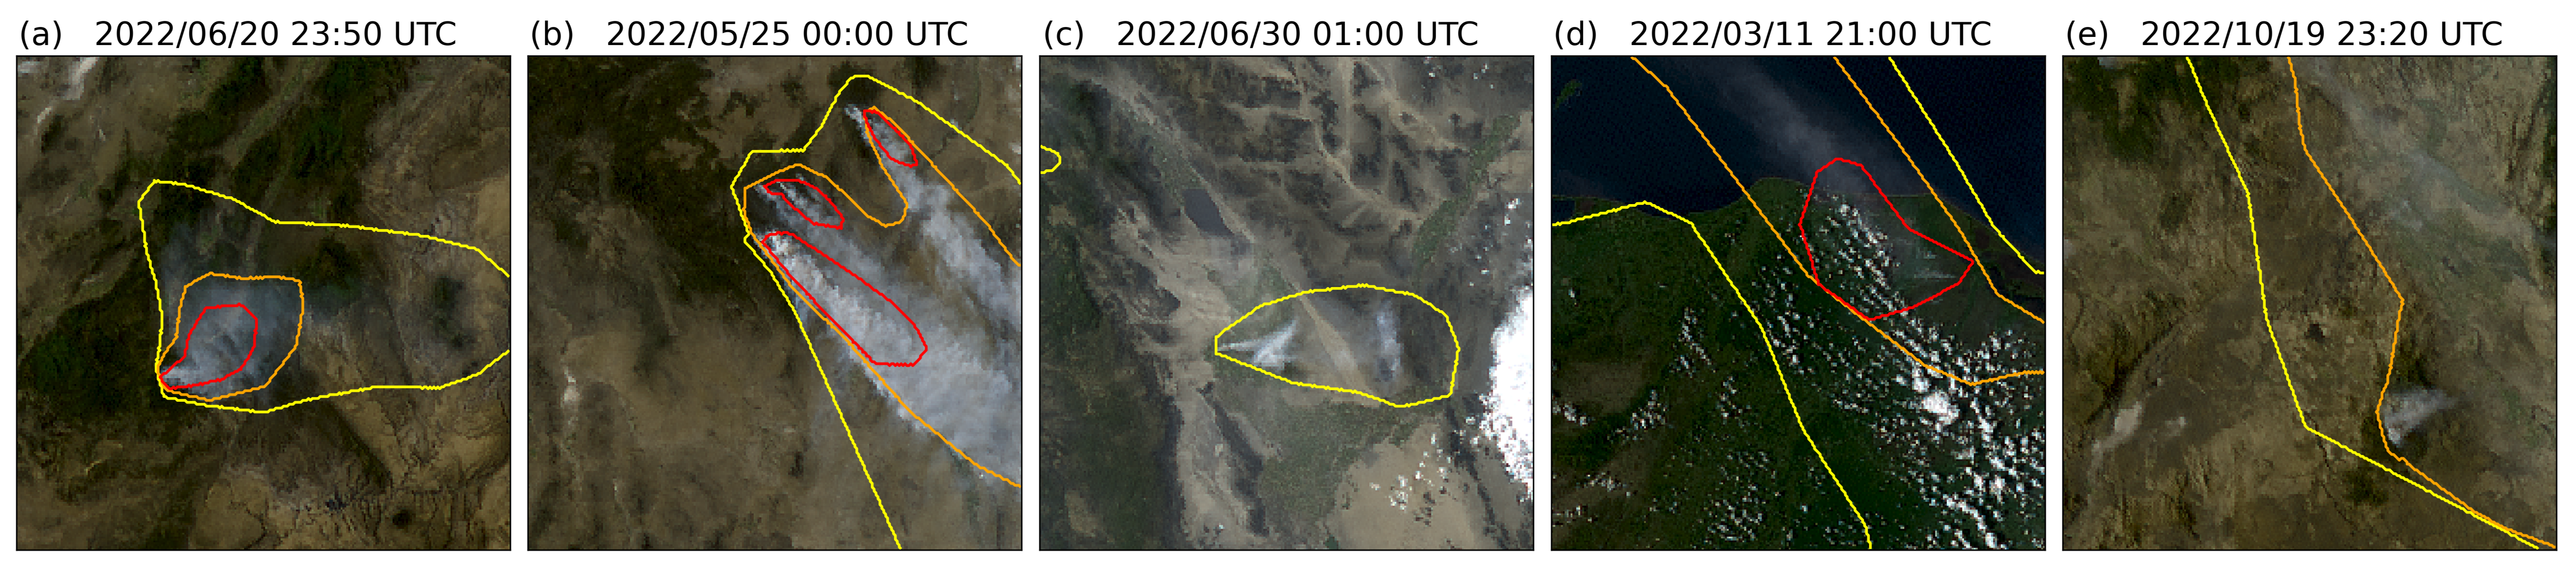
\includegraphics[width=\linewidth]{figures/variations2.png}
    \caption{HMS smoke annotations overlaid on GOES imagery, the yellow, orange and red contours indicate the extent of light, medium and heavy density smoke. (a) and (b) show a canonical examples of a smoke plumes. (c)-(e) show observable variations in the density labels.}\label{densities}
\end{figure*}


\subsection{Introducing a Smoke Analysis Product for Data Assimilation}

The High-Resolution Rapid Refresh (HRRR) model and prototype Rapid Refresh Forecast System (RRFS) produce short-range weather forecasts for CONUS and Alaska, including predictions of wildfire smoke. For each hour, the model is initialized using meteorological data assimilation, combining weather observations with a 3-D model background. While these models use satellite-detected FRP to determine location and smoke emissions associated with wildfires, there is currently no assimilation of smoke observations. We propose to use a deep learning derived smoke identification product to create a smoke analysis to initialize HRRR or RRFS.  

Currently, HRRR and RRFS have a significant latency for representing the plumes from recently started wildfires figure \ref{marshall}.  HRRR relies on polar-orbiting satellites, which only pass over a point on Earth’s surface twice per day.  RRFS uses detections from geostationary satellites, which can detect fires with much lower latency, but depends on the Regional ABI and VIIRS fire Emissions (RAVE) algorithm which takes some time to run.  In addition, formal data assimilation of either satellite aerosol optical depth (AOD) or surface-based smoke observations takes considerable computational time and resources.  For these reasons, a deep learning based smoke analysis could significantly improve short-range model forecasts in rapidly evolving situations featuring new fire starts.  

\begin{figure*}
    \centering
    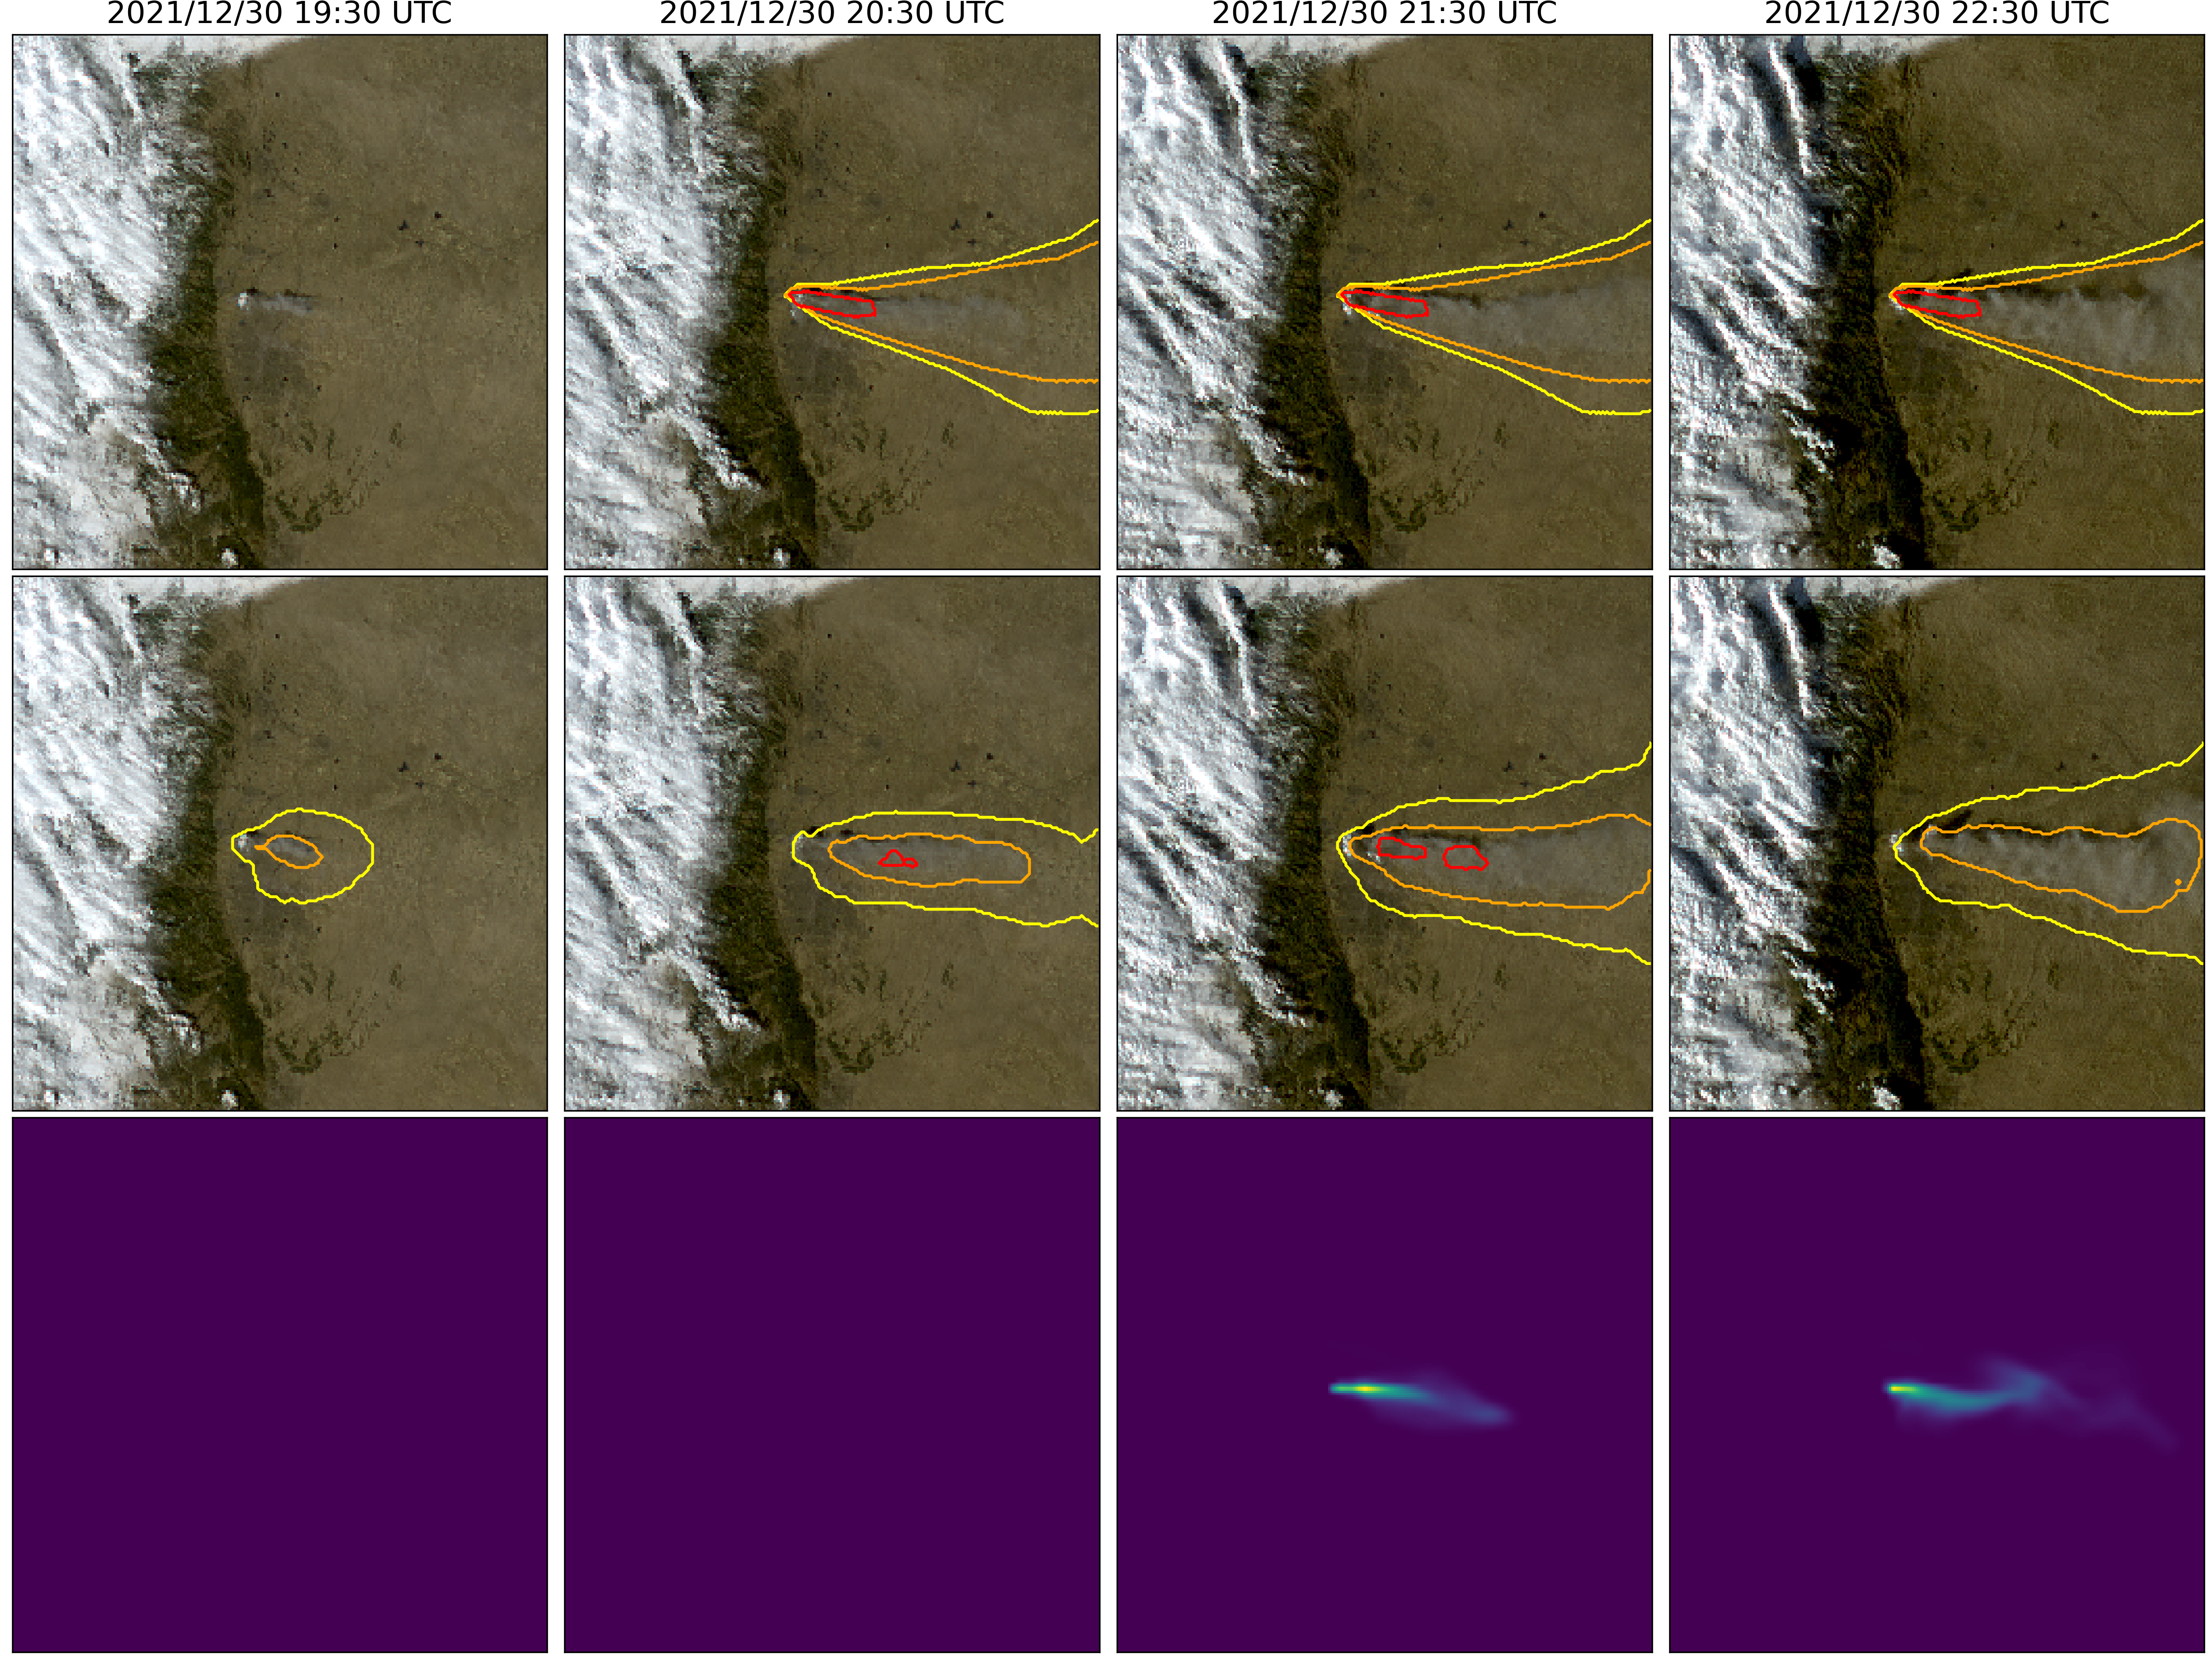
\includegraphics[width=\linewidth]{figures/marshall.png}
    \caption{Top row shows the HMS smoke annotations, middle is SmokeViz and bottom row is HRRR smoke for the start of the Marshall fire in Boulder, CO on December 29th, 2021.}\label{marshall}
\end{figure*}

\section{Methods and Activities}

While we will work directly with the fire weather testbed to develop a thorough and fair proccess for SmokeViz evaluation, here we will provide a summary of key aspects we will address.

\begin{enumerate}
    \item \textbf{Identify all the relevant end users.} We have the HMS analysts that would directly use the product and HRRR/RRFS smoke dispersion model developers, but would want to determine if including further down the line users would be relevant to the evaluation. The HMS smoke product and HRRR forecast is publically published online so that it is difficult to track all users, but we will develop a strategy for identifying and communicating with users.

    \item \textbf{Establish the needs for all end users.} While we have the needs established for those end users that are collaborators on this proposal, we need to perform an assessment on current further down the line end users of the HMS smoke product.

    \item \textbf{Survey how to improve training material and documentation.} We have a tutorial available on how to use the SmokeViz model on specified GOES imagery, but would want to do further assessments on how we can make it more user-friendly to not only the scientific community but also the general public. This would be an iterative proccess that would start before the official testbed evaluation event. Success of the training materials will be included as part of the testbed evaluation.

    \item \textbf{Develop evaluation scenarios.} The SmokeViz model was trained on smoke plumes from 2018-2021 and 2024. 2023 data served to validate the model and 2022 was used for final performance testing. Since neither of those years were used for training the model they could be included for testbed evaluation but it would be important to add in events from 2025 that the model has never touched before. We would need to include scenarios from varying solar zenith angles during the day and over different seasons of the year. Since the SmokeViz model domain covers all of North America, there should be scenarios that span multiple geolocations within those boundaries. While currently untested, we anticipate SmokeViz to have similar performance in the Southern hemisphere and would include samples to test that hypothesis.

    \item \textbf{Perform evaluation.} 

\end{enumerate}


\section{Products/Outputs}
The project will produce an operationally-ready smoke analysis product that can be used for near-realtime DA for air quality models. Additionally, a comprehensive report on the operational utility of the SmokeViz product will be delivered in order to support operational deployment.

Potential end-user adopters of the SmokeViz product would include the scientists that create and run the air quality and smoke plume dispersion models along with down-the-line air quality forecasters and decision makers.

\section{Impacts/Benefits/Outcomes}

The expected result will be an efficient deep learning based smoke analysis product that describes the current extent and categorical density of smoke. Used as a smoke DA product, SmokeViz is expected to significantly advance short-range model predictive capabilities for rapidly evolving wildfires.

\section{Schedule}

\begin{tabular}{ |p{3cm}|p{3cm}|p{8cm}|  }
 \hline
 \multicolumn{3}{|c|}{Schedule} \\
 \hline
 Date & Start RL & milestone\\
 \hline
 Q1 & 5 &AFG\\
 Aland Islands&   AX  & ALA   \\
 \hline
\end{tabular}

The current RL for this project is RL 5 where we have performed evaluation and testing for SmokeViz on streaming GOES imagery. At the end of this project timeline, we will work with a transition partner to reach readiness level 8.

\section{Outreach and Education}

We've developed a series of Jupyter Lab notebooks that walks users through the SmokeViz dataset hosted by NOAA that includes HMS analyst annotations and the corresponding GOES imagery. The notebooks demonstrate how to use the currated dataset to train their own deep learning models and how to apply the tested SmokeViz model to incoming GOES imagery in order to detect active smoke plumes.

\section{Diversity and Inclusion}

The original SmokeViz dataset and model project began during the 2022 NOAA/CIRES summer internship program. This program was a CIRES diversity and inclusion initiative to give underrepresented graduate students opportunities to work with NOAA scientists on GSL research projects. Being queer, Pacific Islander and having aligned research goals with GSL, PI Rey Koki was able to establish collaborations for SmokeViz directly due to this summer intership opporturnity. Now Rey has joined CIRES as a research associate and is able to continue close collaborations at NOAA with the goal of getting SmokeViz operational. Rey Koki is the only member in their direct or extended family to hold a 4-year college degree, yet alone a graduate degree. 

The work towards having SmokeViz ensemble multiple deep learning methods was a result of a collaboration with a summer Hollings undergraduate intern, Annabel Wade. PI Rey Koki and collaborator Jebb Stewart continue to make efforts to facilitate research opportunities to undergraduate and graduate level students.

\section{Data and/or Software Management Plan}

%-------------------------------------------------------------------------


%\section{Related Work}
\label{sec:formatting}


\subsection{Numerical}

Currently, multi-channel thresholding is a popular method to distinguish smoke pixels from pixels containing dust, clouds or other phenomenon with similar signatures \cite{threshold}. Thresholds are determined by using historical, labeled data to extract optimal radiance values for each channel that corresponds with the labeled class. These methods are tuned to particular biogeographies and often have issues with generalization to new locations with varying fuel types \cite{thresh_geog}.

\subsection{Analyst} 
In contrast to the numerical thresholding approach, human visual inspection of satellite imagery is another commonly used method for smoke identification. Trained analyst inspect satellite imagery and label the smoke by hand. An example of hand-labeled annotations is the National Oceanic and Atmospheric Administration (NOAA) Hazard Mapping System (HMS) fire and smoke product \cite{hms, hms_val}. For the HMS smoke product, trained satellite analysts use movement characteristics to help identify smoke by scanning through a time series of satellite imagery. When visual inspection indicates smoke, the analyst will draw a polygon that corresponds to the geolocation and density of smoke. By design of the product, the HMS annotations have varying time resolution and are released on a rolling but undefined schedule ranging from one to multiple times a day as observation conditions permit. If expanded beyond the current North American boundary, this method will not be as scalable as an automated approach and is limited by the availability of analysts and their time. 

NOAA manages environmental satellite programs such as the HMS program, an operational system that uses an aggregation of satellite data to generate active fire and smoke data. To train our model, we implement a supervised learning framework that uses the HMS analyst smoke product as truth labels during the model training process.

HMS smoke analysis data gives the coordinates of the smoke perimeter as a polygon and classifies the smoke by density within a given time window. The time windows can range from instantaneous (same start/end time) to lengths of 22 hours. While the true bounds of the smoke can change within the larger time spans, the analyst is making an approximation that should reflect the smoke coverage over the duration of the time window. The density information is qualitatively determined by each analyst based on the apparent smoke opacity in the satellite imagery and categorized as either light, medium or heavy as seen in figure \ref{densities}a \cite{hms_web}.

\subsection{Deep Learning}

To address the challenges associated with thresholding and manual labels, we can look towards innovative approaches and recent technological advancements in computer vision. Machine learning methods have shown potential in improving the accuracy and efficiency of satellite-based wildfire smoke detection and monitoring. For instance, SmokeNet, uses a convolutional neural network (CNN) based framework to determine if a scene of MODIS satellite imagery contains smoke \cite{smokenet}. Another study, that looked at a singular wildfire event, also used a CNN to identify smoke on a pixel-wise basis using imagery from Himiwari-8 \cite{larsen}. Additionally, Wen et al. developed a CNN architecture that takes GOES-East imagery as input and the HMS-generated annotations for the target labels during training \cite{smoke_goes}. 

The success of deep learning methods, such as CNNs, relies heavily on the availability of a large, representative dataset \cite{data_size}. As laid out in table \ref{studies}, prior studies use relatively small numbers of samples, from 47 \cite{wang} to 6825 \cite{smoke_goes}, where one sample represents a satellite image with a singular time and geolocation. In contrast, benchmark datasets for image classification contain tens of thousands (CIFAR-10 \cite{cifar} and MNIST \cite{mnist}) to millions (CIFAR-100 and ImageNet \cite{imgnet}) of data samples. Keeping in mind the correlation between both the quality and quantity of data with model performance, we introduce the largest known smoke dataset, SmokeViz, containing over 180,000 samples.

\begin{table*}[h]
    \caption{Comparison of different studies including method used, dataset size, satellite source, number of channels used and if classification is performed at a pixel or image level.}\label{studies}
    \centering
    \begin{tabular}{ccccrrcrc}
        \toprule
        Reference & Method & \verb|#| Samples & Satellite & \verb|#| Channels & Level\\
        \midrule
        \cite{smokenet}& CNN & 6255 & MODIS & 5 & image\\
        \cite{smoke_goes}& CNN & 6825 & GOES-East & 5 & pixel\\
        \cite{larsen} & CNN & 975 & Himiwari-8 & 7 & pixel\\
        \cite{wang}& U-Net & 47 & Landsat-8 & 13 & pixel\\
        SmokeViz  & U-Net & 183,672 & GOES-East/West & 3 & pixel\\
        \bottomrule
    \end{tabular}
\end{table*}

Semi-supervised learning is an approach that can be used to increase the number of labeled samples in a dataset. This is done by leveraging a labeled dataset to generate new labels for an often larger, but unlabeled, dataset. Pseudo-labeling, a form of semi-supervised learning, uses labeled data to train an initial model, then runs that model on unlabeled data to predict pseudo-labels, and finally trains a new model using the pseudo-labels \cite{pseudo}. Since we do not know of any studies that have used this technique in this way, we introduce a variation of pseudo-labeling, not to increase the size, but to increase the quality of our dataset by generating pseudo-labels to select the best satellite image out of a given time-window to represent each smoke plume annotation.

\begin{figure*}
    \centering
    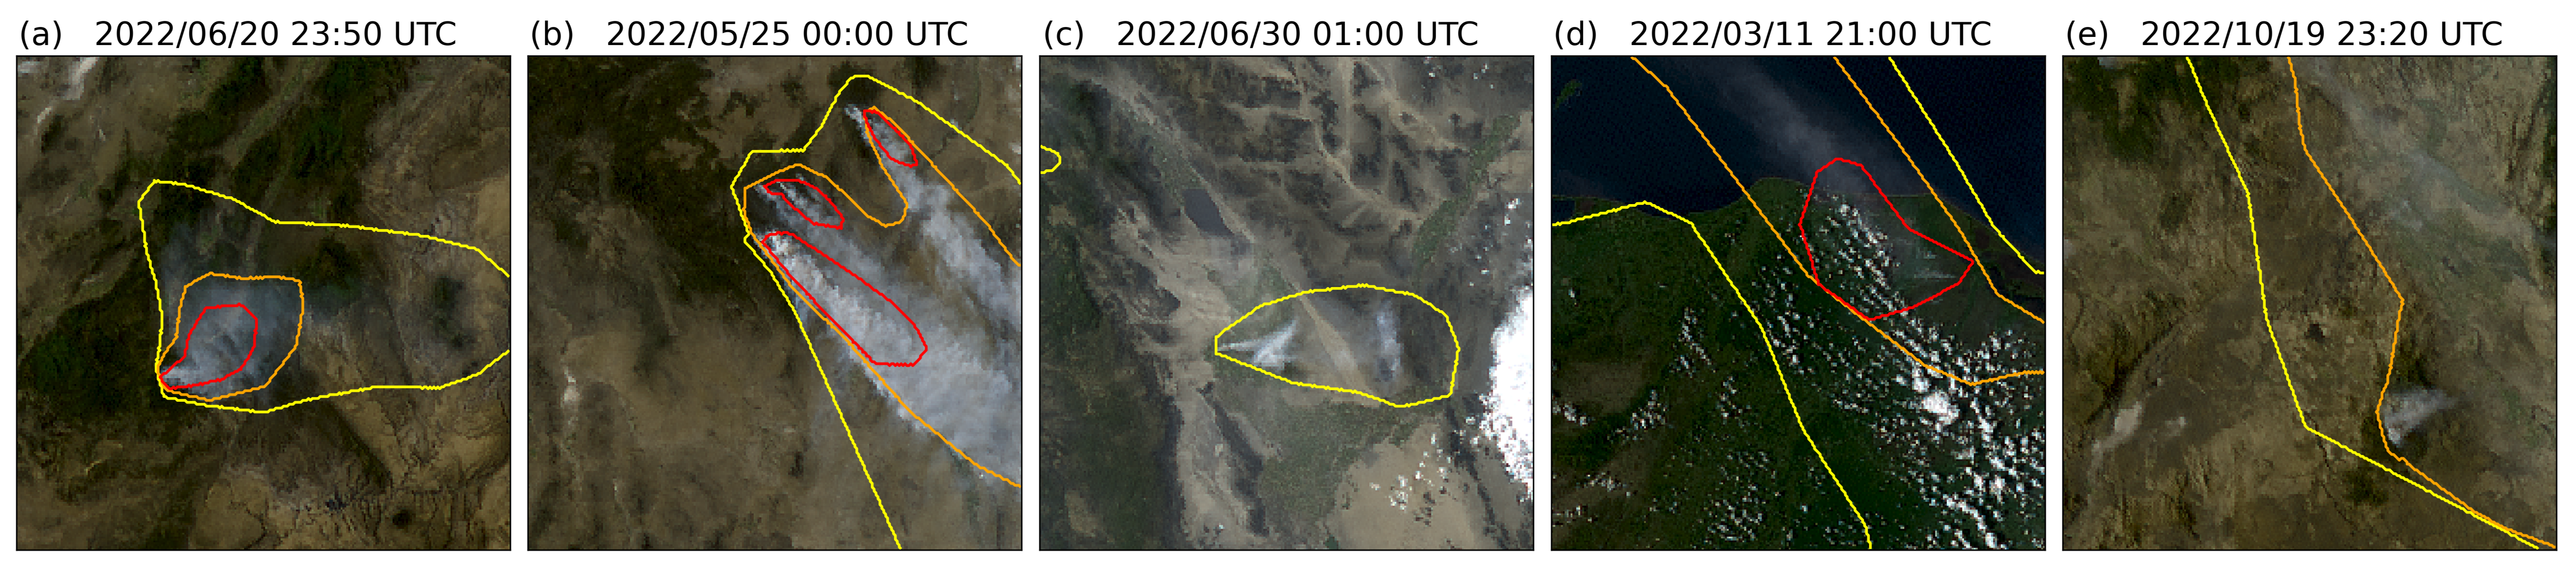
\includegraphics[width=\linewidth]{figures/variations2.png}
    \caption{HMS smoke annotations overlaid on GOES imagery, the yellow, orange and red contours indicate the extent of light, medium and heavy density smoke. (a) and (b) show a canonical examples of a smoke plumes. (c)-(e) show observable variations in the density labels.}\label{densities}
\end{figure*}


%$\section{Methods}
\label{sec:formatting}
\subsection{Datasets}

In order to take into account movement characteristics to help identify smoke, analysts use multi-frame animations of the satellite imagery. The resulting annotations primarily have time windows over multiple hours, with an average of 3 hours of imagery represents one smoke plume annotation. Since the goal of these annotations is to show the general coverage over that time span, as shown in figure \ref{timelapse}, the smoke boundaries don't often match up with the satellite imagery over the entire time window. One way to approach this problem would be to use all the satellite images the analysts used as input. Since the timespans are non-uniform, this would vary the length in imagery inputs into the model, which would be difficult with a CNN architecture. Moreover, this would require a large amount of additional memory and computational resources. Instead of using the original analysts' many satellite image inputs to one annotated output, we develop a one-to-one input-to-output by finding the optimal singular satellite image input to represent the annotation. 

\begin{figure*}
    \centering
    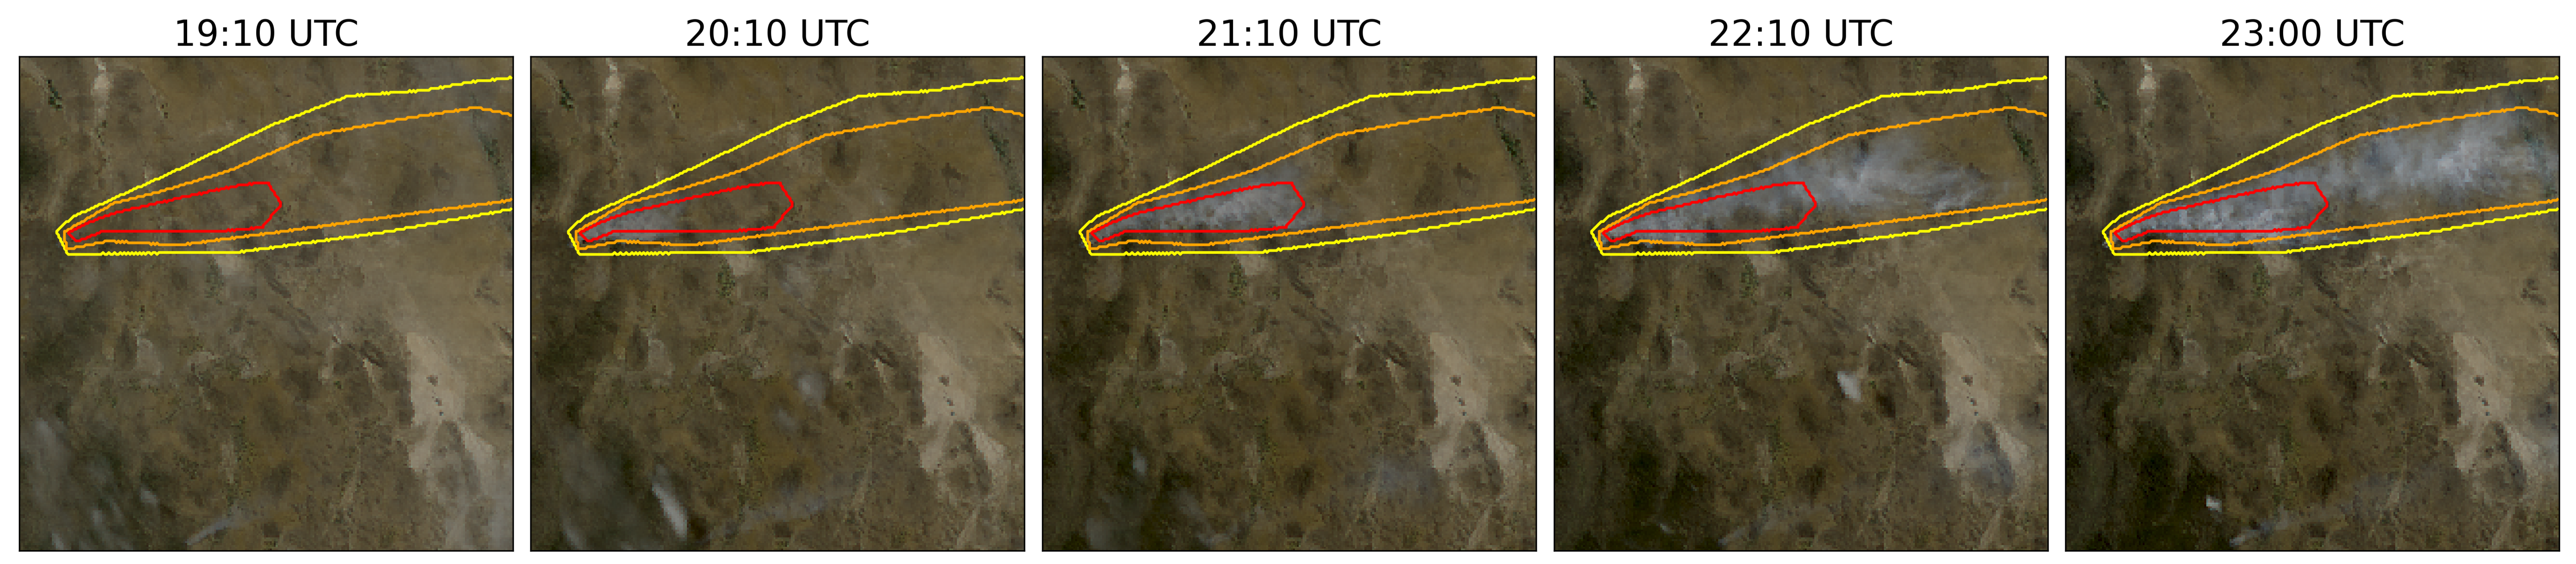
\includegraphics[width=\linewidth]{figures/TIMELAPSE_FINAL2.png}
    \caption{True color GOES-East imagery from May 5th, 2022, Southeast New Mexico (\(31.38^{\circ}\)N, \(107.87^{\circ}\)W) during the start of the Foster Fire. The red, orange and yellow lines represent the heavy, medium and low density HMS smoke annotations that span 19:10\textendash23:00 UTC.}
    \label{timelapse}
\end{figure*}



For the set of smoke annotations, \(\mathcal{Y}\), \(y \in \mathcal{Y}\) uses one or more \(x \in \mathcal{X}\) where \(\mathcal{X}\) is the entire set of satellite imagery corresponding to the set of time windows defined by the labels. In order to develop a one-to-one data-to-label dataset, we apply pseudo-labeling to develop a subset of \(\mathcal{X}\), denoted as \(\mathcal{X}_p\), that has a one-to-one ratio such that \(|\mathcal{X}_p| = |\mathcal{Y}|\), where we choose the satellite image that has the maximum overlap between the geolocation of smoke in the imagery and the analyst annotation.

But in order to create pseudo-labels we need an initial parent model, \(f_{\circ}\). To train \(f_{\circ}\), we need a way of choosing \(x \in \mathcal{X}\) that has a higher chance than random selection of being representative of \(y\). Discussed in further detail in the Mie-Derived Dataset subsection, we do this by making a series of physics-driven choices on which satellite and timestamp would give the optimal angle between the sun, smoke and satellite to produce the strongest smoke signature for the geolocation and timestamp of the smoke plume. This dataset, \(\mathcal{X}_M\) tells us that if there is smoke present during the entire time window, which timestamp would give the highest smoke signal-to-noise ratio. 

But more importantly than knowing the timestamp for maximum signal-to-noise, we want to know which image actually has smoke present within the smoke label boundaries. We used \(\mathcal{X}_M\) to train \(f_{\circ}\), to identify smoke in satellite imagery, and then use that \(f_{\circ}\) to create pseudo-labels of each satellite image in a given annotation's time-window. From those results, the optimal satellite image is chosen based on which image's pseudo-labels has the greatest overlap with the analyst annotation.




\subsubsection{Satellite Imagery} 

The GOES satellites are operated by NOAA in order to support meteorology research and forecasting for the United States. We use the latest operational satellites, GOES-16 (East), 17 and 18 (West) that each carry the ABI, that measure 16 bands between the visible and infrared wavelengths. In improvement to the GOES predecessors, imagery is collected every 5 minutes for the contiguous United States and every 10 minutes for the full disk. Using PyTroll, a Python framework for processing satellite data \cite{satpy}, we input bands 1-3 (Table \ref{rgb_bands}) to a GOES specific true color composite algorithm \cite{true_color} to develop a, 1km resolution, true color image representation, similar to what is seen by HMS analysts. As discussed in further detail in the next section, the highest signal-to-noise ratio will come from the smallest wavelengths of light, larger wavelengths have lower smoke signal and higher noise (figure \ref{bands}). For that reason, we only include the first 3 out of 16 available bands of data.

\begin{table}
    \caption{To create a true color image, we use the following bands from the ABI Level 1b CONUS (ABI-L1b-RadC) product.}\label{rgb_bands}
    \centering
        \begin{tabular}{ccccrrcrc}
            \toprule
            band & description & center \(\lambda\)($\mathrm{\mu m}$) & resolution (km)\\
            \midrule
            C01 &  blue visible & 0.47 & 1 \\
            C02 & red visible & 0.64 & 0.5 \\
            C03 & veggie NIR & 0.865 & 1 \\
            \bottomrule
        \end{tabular}
\end{table}


\subsubsection{Mie-Derived Dataset}

We used a physics-informed approach in selecting the initial GOES dataset, \(\mathcal{X}_M\), which we call the Mie-derived dataset, for training an initial parent model, \(f_{\circ}\), where if \(\mathcal{X}\) represents all the GOES imagery corresponding to the HMS smoke annotation time window, \(\mathcal{X}_M \subset \mathcal{X}\). Prior GOES ABI datasets for machine learning applications often include data from only one of the two GOES-series satellites, commonly opting for GOES-East \cite{smoke_goes}, \cite{wildfire_detect}, \cite{goes_conv}. Rather than using one satellite or the cumulative data from both GOES-West and GOES-East images, we select between one or the other based on the solar zenith angle. For smoke identification, this approach can achieve a much higher signal-to-noise than imaging the earth’s surface from an arbitrary angle. The elastic scattering of light is the primary mechanism to account for - while the atmosphere is composed of molecules with size \(<\)1nm, smoke particles can vary from 100 nm -- 10 \(\mu\)m in diameter, \(d\). The GOES ABI covers spectral bands from 0.47 \(\mu\)m -- 13.3 \(\mu\)m, so atmospheric and smoke particle sizes occupy two very different regimes with respect to the imaging wavelength \(\lambda\). In the extreme limit of \(\lambda \gg d\), the physics of scattering of light off a small sphere is captured by Rayleigh scattering. This process has two critical consequences: (1) the scattering cross section of light is strongly wavelength dependent (scaling with \(\lambda^{-4}\)), meaning that photons with wavelength closer to the ultraviolet are scattered more strongly than infrared photons. (2) the scattering cross section scales with an angular dependent cross section of \((1 + \cos^2 \theta)\). Scattered photons follow the emission distribution of a radiating dipole, scattering more strongly in the forward and backwards directions \((\theta = 0,\pi)\)than orthogonal to the direction of propagation \((\theta = \pi/2, 3\pi/2)\), see figure \ref{mei} for a Rayleigh scattering schematic.


\begin{figure}
    \centering
    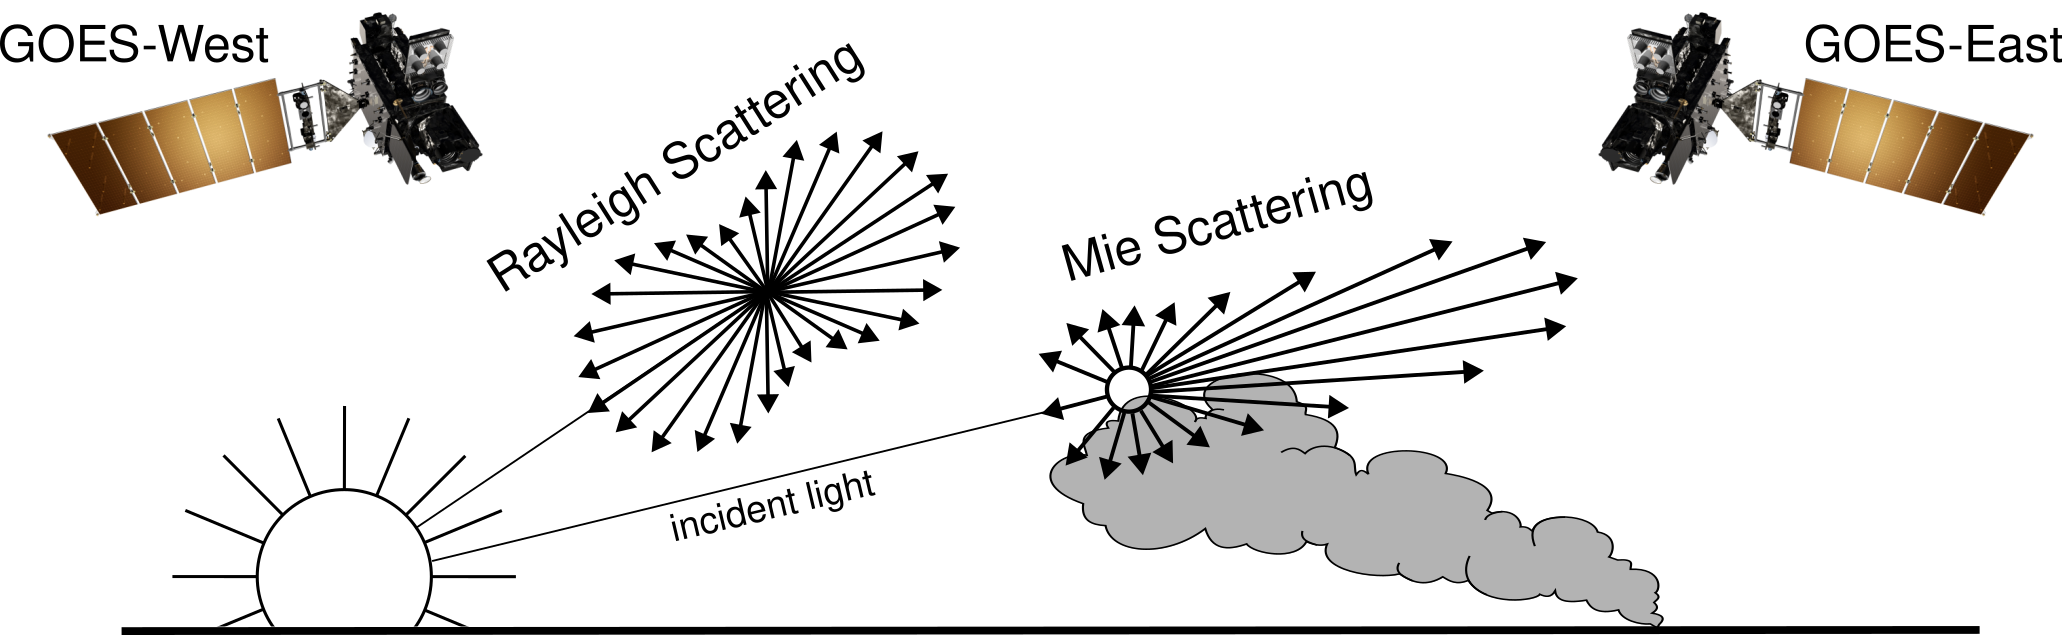
\includegraphics[width=8cm]{figures/mei.png}
    \caption{If the particle size is \(<\frac{1}{10}\) the wavelength of the interacting light, then the primary scattering will be Rayleigh. Mie scattering is the predominant scattering mechanism when the particle size is larger than the wavelength of light. This schematic demonstrates that when the sun is setting in the West, the Mie scattering will predominately forward scatter towards GOES-East.} \label{mei}
\end{figure}

The significance of these scalings is that the observer, or detector, will receive blue photons in most directions orthogonal to the source. Equivalently, photons traveling colinearly with line of sight to the emission source will mostly have wavelengths in the infrared band. In the converse regime of \(d > \lambda\), the elastic scattering of light against matter is modeled through Mie scattering. In comparison to Rayleigh scattering, Mie scattering is largely wavelength-independent and has a more complicated radiation pattern where the cross section has a maximal amplitude in the forward direction. An observer downstream of this scatterer will collect more photons than one positioned directly behind it. In the context of smoke identification, a sunrise or sunset will lead to a higher Mie scattered signal in GOES-West and GOES-East respectively, as shown with a smoke plume producing a stronger signal in GOES-East imagery near sunset in figure \ref{16_vs_17}.

\begin{figure}
    \centering
    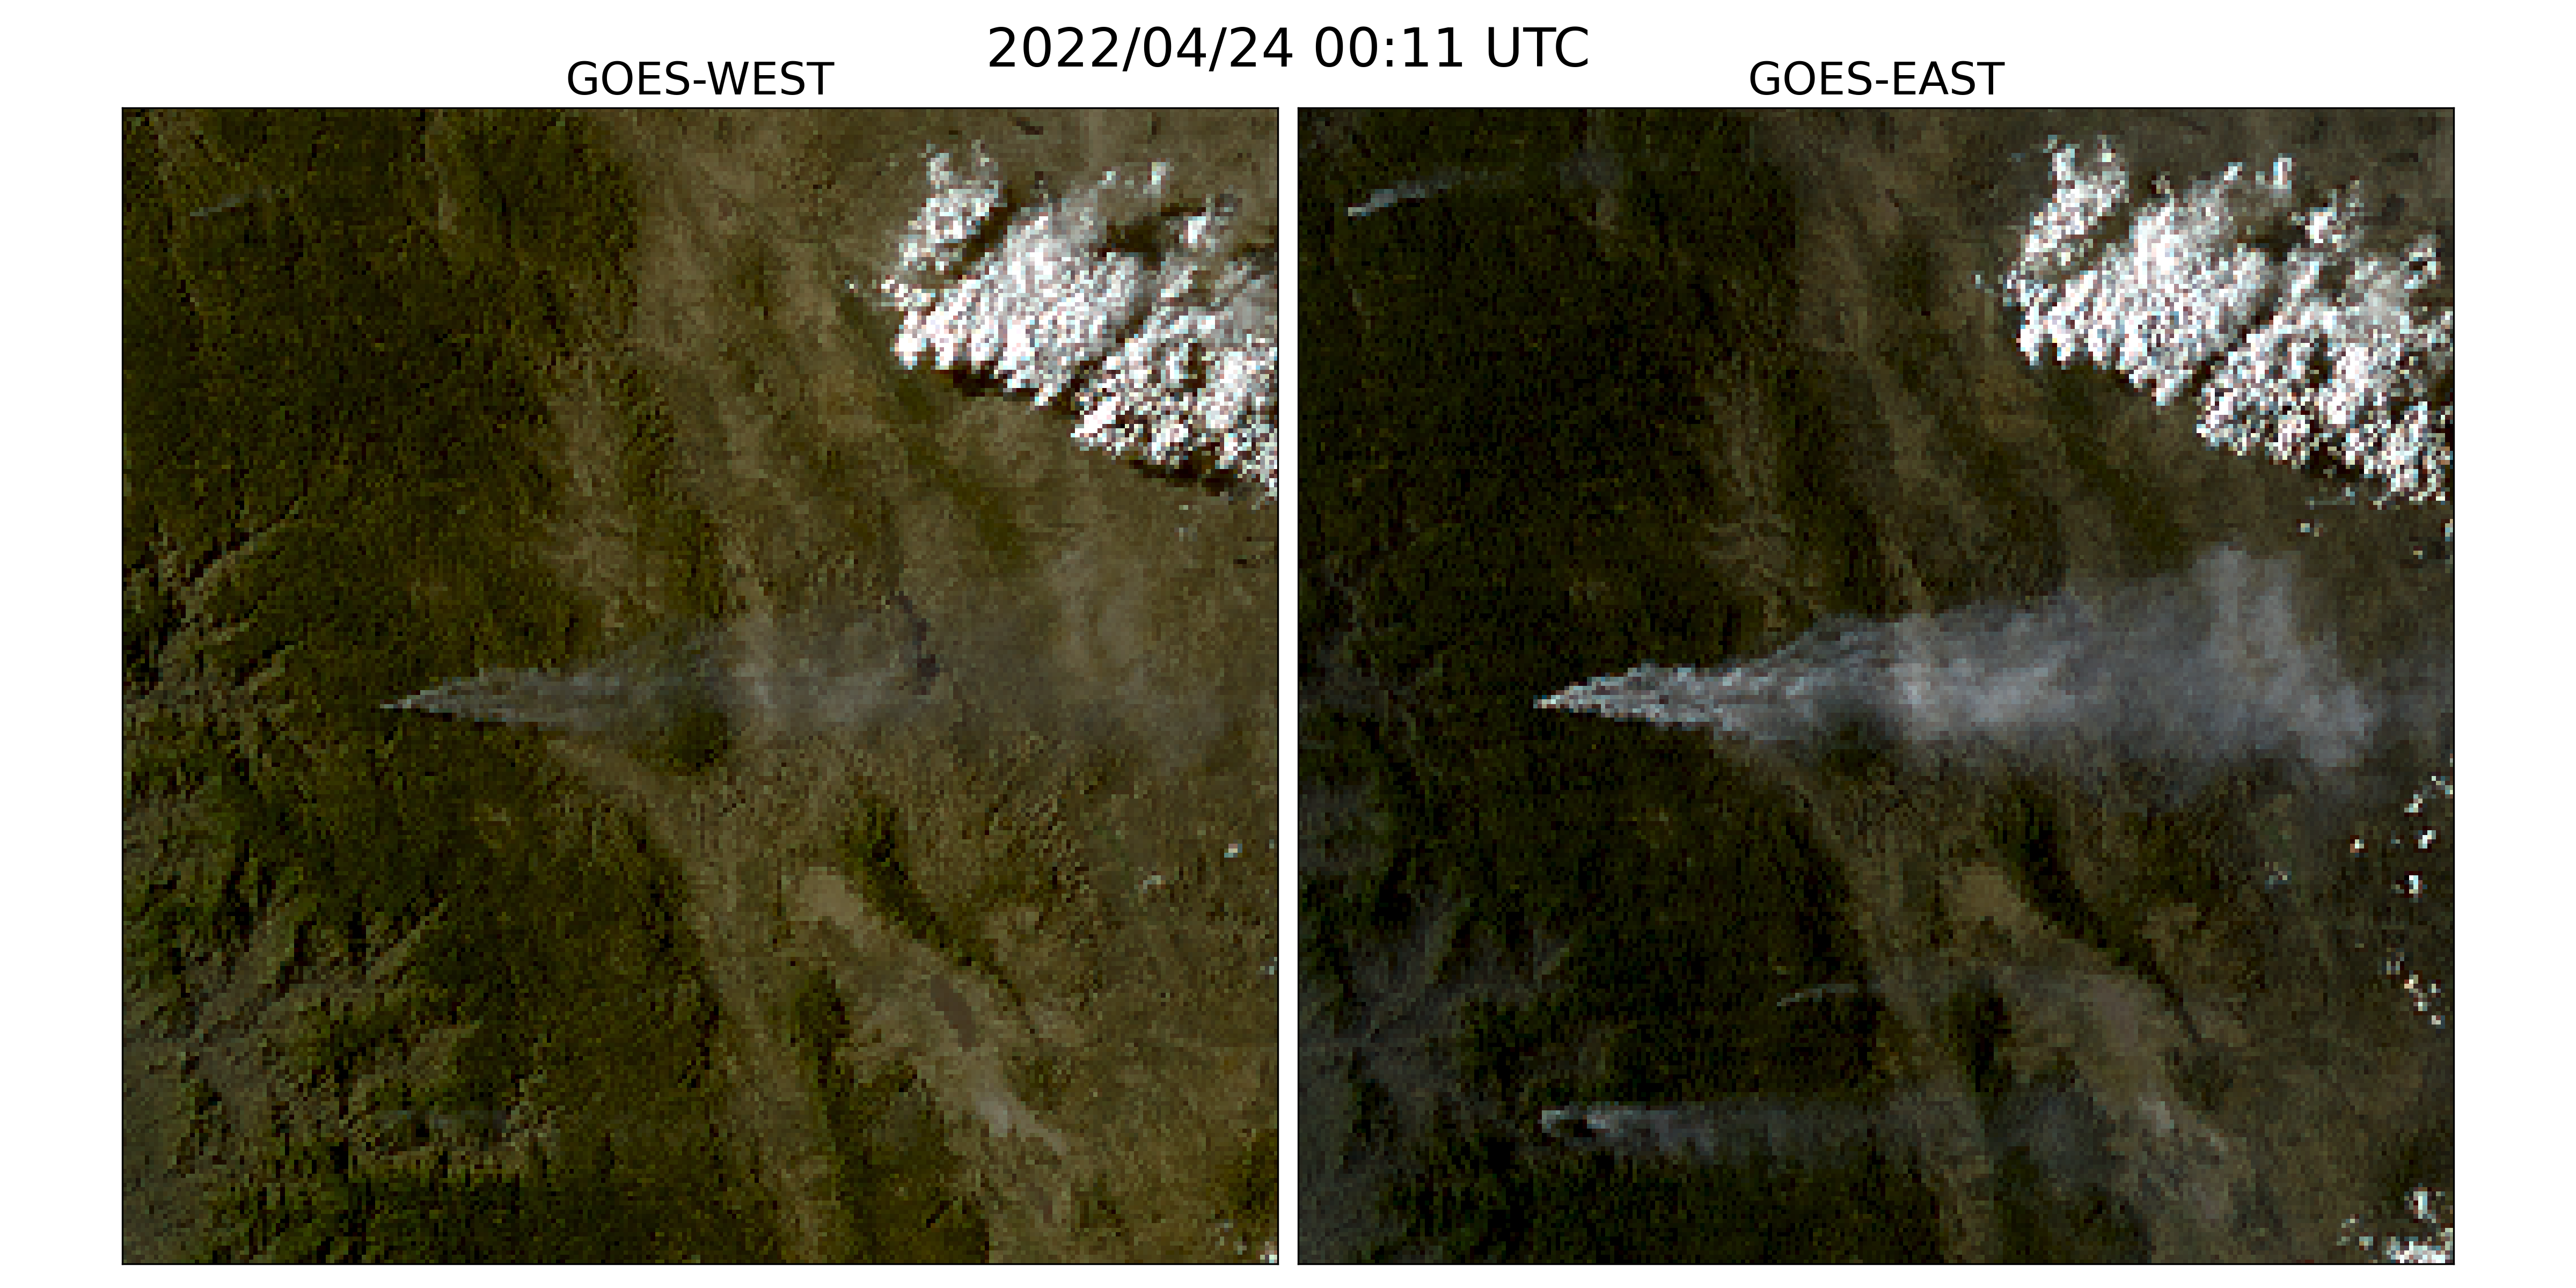
\includegraphics[width=8.5cm]{figures/G16_v_G17_2.png}
    \caption{True color GOES-West (left) and GOES-East (right) imagery from April \(24^{th}\), 2022 in Durango, Mexico. The images were taken \(\sim1.5\) hours before sunset (01:43 UTC) for this geolocation and time of year.}\label{16_vs_17}
\end{figure}

Smoke identification therefore amounts to extracting a signal of \(d > \lambda\) photons from the \(\lambda \gg d\) background. Positioning a detector along line of sight to the scatterer will result in a higher signal from smoke particles (figure \ref{mei}). Filtering the imaged wavelength can enhance this signal; photons collected in the blue spectrum will have a naturally lower background along the line of sight to the illumination source do their high level of Rayleigh scattering as. Therefore, as demonstrated in figure \ref{bands}, this configuration results in the highest signal to noise imaging for smoke particles.

\begin{figure}
    \centering
    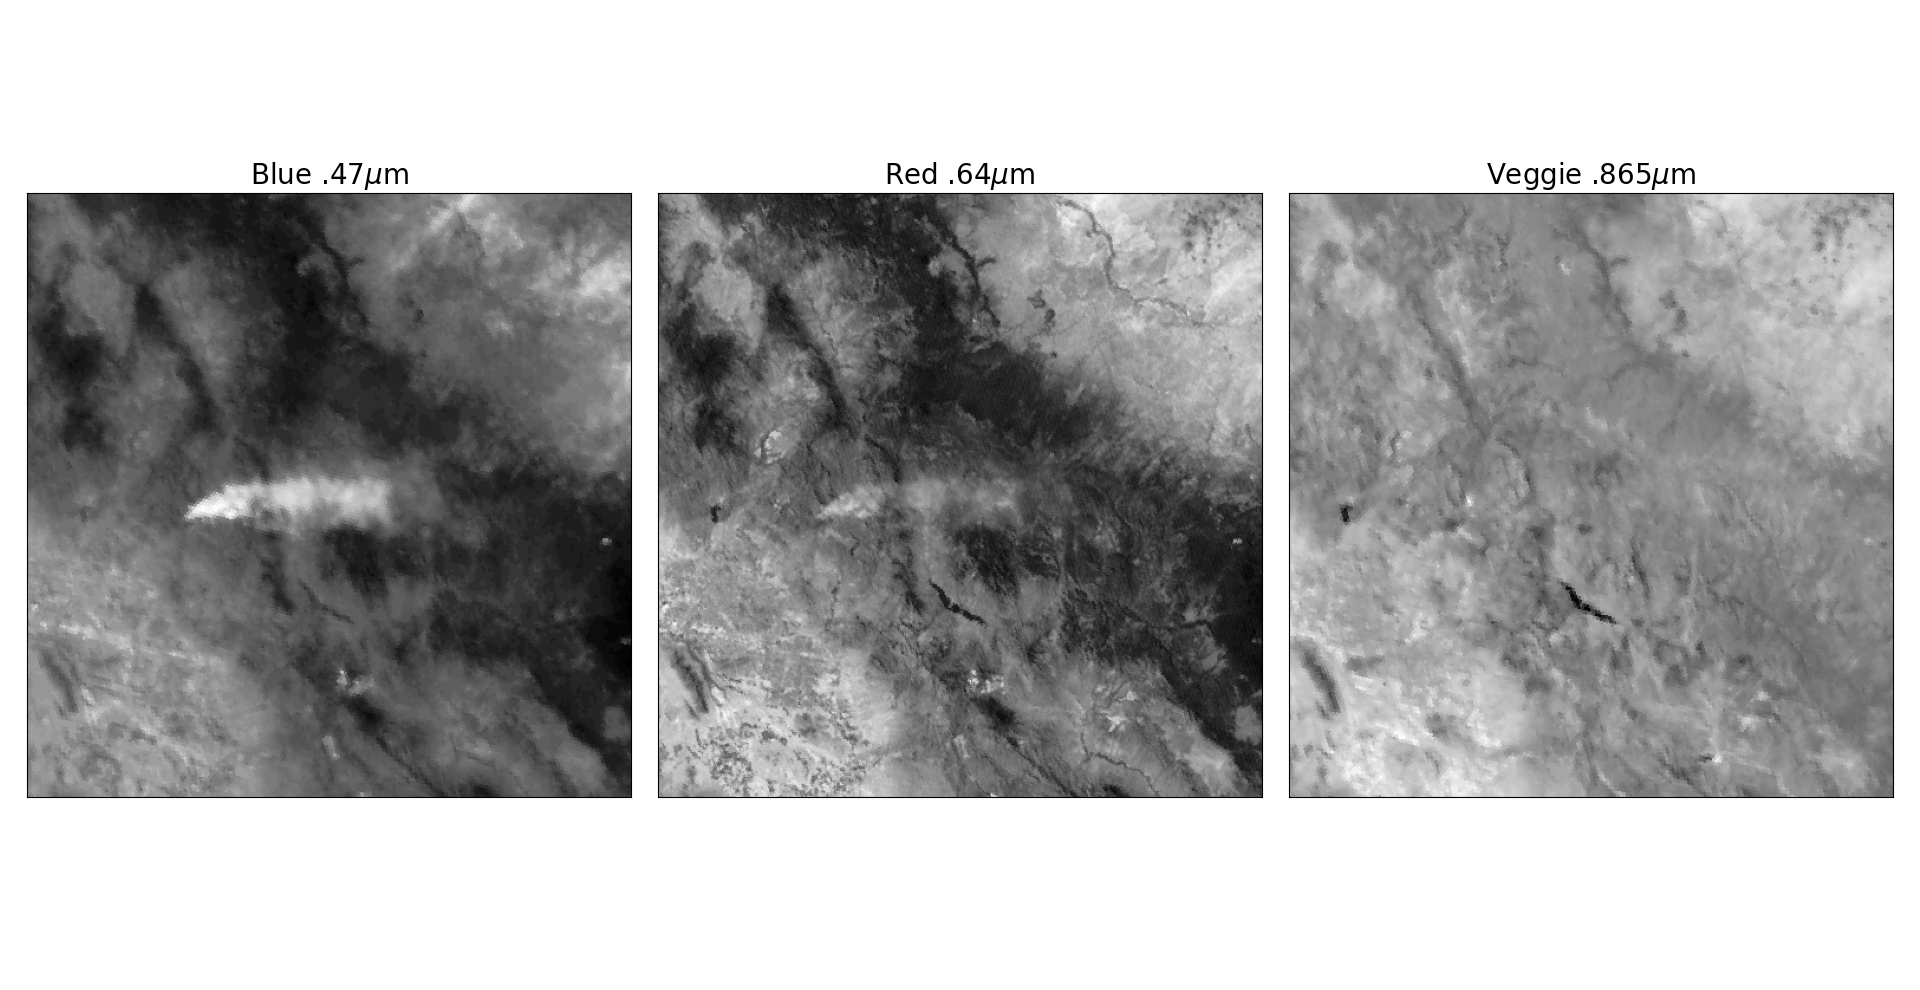
\includegraphics[width=8cm]{figures/GOES16_bands.png}
    \caption{Three bands of GOES-East data are the raw input to generate a true color image. These plots show variations in the signal-to-noise ratio for smoke detection in relation to the \(\lambda\) of light being measured.}\label{bands}
\end{figure}

Based solely on these criteria, the optimal strategy would be to pull data from GOES-West right after sunrise and from GOES-East right before sunset. Another factor to consider is that the time when the sun is in optimal alignment with the satellite for smoke detection coincides with when solar zenith angle is close to \(90^{\circ}\). Larger angles between the satellite and sun result in an increase in noise due to increased atmospheric interactions \cite{zen_angle}. To reduce the noise from large solar zenith angles, if given multiple frames to choose from, we choose the image with the largest solar zenith angle that is \(<88^{\circ}\).

The resulting image selection process takes into account atmospheric properties and light scattering physics to generate an estimate of which singular satellite image within the analyst time-window could give the highest smoke signal-to-noise ratio. The resulting Mie-derived dataset, \(\mathcal{X}_M = \{X_M, Y\}\), was then used to train a model, \(f_{\circ}\), that would generate \(N\) pseudo-labels, \(y^*\), for every sample, where \(N\) is determined by how many images, taken at a 10 minute interval, fit within the analyst time-window for that sample. Chosen from the \(N\) images, \(x_p\) is the image with the highest alignment between the \(f_{\circ}\) prediction of smoke, \(y^*\), in the image and the HMS analysts' annotation \(y\).

\subsubsection{Thermometer Encoding Smoke Densities}

One of the challenges introduced with using human generated qualitative smoke densities was that, as seen in figure \ref{densities}(c)-\ref{densities}(e) , there are variations in what is labeled as heavy or light density smoke. More generally, reproducing qualitative metrics with quantitative algorithms is a challenging problem, but we apply mathematical approaches that mitigate some of the underlying complications of our specific problem. Despite the smoke densities introduce qualitative complexities, we decided that the density approximations were important to use in our dataset because of the differences in signatures the densities produce. Within the satellite imagery, the appearance of a light density smoke plume will look significantly different than a heavy density smoke plume as seen in figure \ref{densities}. Additionally, a light density smoke plume is expected to be more challenging to detect since it is easier for it to be misclassified as not smoke. During the training process, the separate density categories allows us to deferentially weight the penalization given to the model for incorrect classifications based on category. For example, the model can be given a small penalization for misclassifying light smoke as not smoke while given a higher penalization for misclassifying heavy smoke as not smoke. 

In addition to the densities being ordered and categorical, the differences between the density categories are not evenly distributed by a given metric, such as PM\textsubscript{2.5} density. The intervals between densities being unknown along with the hierarchical nature of the density labels makes the labels ordinal instead of just categorical. This data property allows us to use thermometer encoding \cite{therm_enc}, which leverages the idea that heavy density smoke includes both medium and light density smoke, that heavy density smoke is closer to medium than it is to light, and automatically weights the loss functions and incorporates the ranked ordering of the densities. As seen in Table \ref{therm}, one-hot encoding, commonly used for categorical data, doesn't take ordinal properties of the data into consideration.

\begin{table}[h] 
    \caption{A comparison of one-hot encoding used for categorical data to thermometer encoding for ordinal data.}\label{therm}
    \centering
    \begin{tabular}{ccccrrcrc}
        \toprule
        category & one-hot & thermometer \\
        \midrule
        No Smoke & \texttt{[0 0 0]} & \texttt{[0 0 0]} \\
        Light  & \texttt{[0 0 1]} & \texttt{[0 0 1]} \\
        Medium & \texttt{[0 1 0]} & \texttt{[0 1 1]} \\
        Heavy  & \texttt{[1 0 0]} & \texttt{[1 1 1]} \\
        \bottomrule
    \end{tabular}
\end{table}

\subsubsection{Pseudo-label Dataset} 

We implement a deep learning architecture that uses the encoder from EfficientNetV2 \cite{efficientnetv2} and a semantic segmentation classifier from the DeepLabV3 model \cite{deeplab}. Transfer learning has shown to reduce the time and resources needed to train a model by leveraging information from pre-trained models \cite{transfer}, \cite{transfer2}. We initialize the values of our model weights using the pre-trained values originally trained on the ImageNet dataset \cite{imgnet}, containing 1.2 million images and 1000 categories. Our model was developed using the Segmentation Models PyTorch package \cite{semantic} that was written as a high level API for implementing models for semantic segmentation problems. We input 256x256x3 snapshots of 1km resolution true color GOES imagery that contains smoke and output a 256x256x3 classification map that predicts if a pixel contains smoke and if so, what the density of that smoke is. As mentioned earlier, we apply the thermometer encoding shown in table \ref{therm} to encode the smoke densities and apply binary cross entropy as the loss function per density of smoke. 

The dataset, \(\mathcal{X}_M\), contains 207,106 samples as shown in the dataset split in table \ref{split}. 

\begin{table}[h] 
    \caption{Dataset split for \(\mathcal{X}_M\) and \(\mathcal{X}_p\), samples for 2024 go up to November 1st. We use an entire year of data for both validation and testing sets to capture year-long wildfire trends.}\label{split}
    \centering
    \begin{tabular}{ccccrrcrc}
        \toprule
        dataset & \(\mathcal{X}_M\) & \(\mathcal{X}_p\) &years\\
        \midrule
        training & 165,609 & 144,225 &2018-2021, 2024\\
        validation & 20,056 & 19,223 &2023 \\
        testing & 21,541 & 20,224 & 2022 \\
        \bottomrule
    \end{tabular}
\end{table}

To determine which image out of the relevant imagery for the given time window best represents the analyst annotation, we implement a greedy algorithm by running \(f_{\circ}\) on each \(x\) to generate a pseudo-label, \(y^*\). The output of \(f_{\circ}\), \(y^*\) give predictions on if smoke is in the image, and if there is smoke, where the smoke is in that image and the density of that smoke. \(y^*\) serve as pseudo-labels for each density of smoke and are compared to the analyst annotations, \(y\). To compare \(y^*\) and \(y\), we calculate the IoU using the total set of pixels for \(y^*\) at that density of smoke and the entire set of pixels for \(y\) for a particular smoke density in each image as shown in equation \ref{overall_iou}. The image with the highest IoU score is chosen as the image, \(x_p\), that best represents the analyst smoke annotation, \(y\). Often used for pseudo-labeling, a confidence threshold value is defined to determine if a pseudo-label should to be included in a dataset \cite{conf_thresh}. We chose a confidence threshold that would include the sample, \(x_p\), in \(\mathcal{X}_{p}\) if the maximum overall IoU (equation \ref{overall_iou}) between \(y^*\) and \(y\) over all densities was over 0.01. 

\begin{equation} \label{overall_iou}
    IoU_{\text{overall}} = \frac{\sum\limits_{i=\text{light}}^{\text{heavy}}|y_{i}\cap y^*_{i}|}{\sum\limits_{i=\text{light}}^{\text{heavy}}|y_{i}|\cup|y^*_{i}|}
\end{equation}

We use \(\mathcal{X}_{p}\) to train an additional child model, \(f_c\) in order to assess if training with \(\mathcal{X}_{p}\) can produce a more robust semantic segmentation model compared to training on \(\mathcal{X}_M\). We use the same dataset split method and model setup but change \(\mathcal{X}_M\) to \(\mathcal{X}_{p}\) to train \(f_c\).

\subsection{Benchmark Models}

While this dataset is anticipated to be primarily useful for solving various wildfire smoke applications, this dataset could be a uniquely insightful test case for remote sensing semantic segmentation. Many deep learning satellite image datasets are focused on objects with sharp contrasts such as crops \cite{crops}, human infrastructure \cite{polyworld}, or even clouds over oceans \cite{cyclone, cloud_texture}, but smoke has indistinct boundaries that often fade both spatially and temporally.

We benchmark the SmokeViz dataset, \(\mathcal{X}_{p}\) by varying the semantic segmentation classification heads. We train Linknet \cite{linknet}, PSPNet \cite{pspnet} and MANet \cite{manet} using the same encoder used for \(f_c\) and \(f_{\circ}\), EfficientNetV2. Each model is trained over 100 epochs using a batch size of 32 and the Adam optimizer on 8 Nvidia P100 GPUs allocating 100GB of memory over 12 hours of allotted training time. We choose these architectures because of their abilities to capture multi-scale objects such the varying spatial extents of smoke plumes.




%\section{Results}
\label{sec:formatting}

To interpret the performance of \(f_{\circ}\), we report the IoU metrics in table \ref{iou_results} that were computed by running \(f_{\circ}\) and \(f_c\) on \(\mathcal{X}_M\) and \(\mathcal{X}_{p}\). For each density, we calculate the IoU using the total set of pixels that \(f_{\circ}\) predicts as that density of smoke and the entire set of pixels labeled by the analyst as a particular smoke density over all imagery contained in the testing dataset. Additionally, we compute the overall IoU for all densities by first computing the number of pixels that intersect their corresponding density and divide that by the total number of pixels that make up the union of model predicted and analyst labeled smoke in the testing dataset.

\begin{table} 
    \caption{IoU results per density of smoke and over all densities using \(f_{\circ}\) and \(f_c\) with \(\mathcal{X}_M\) and \(\mathcal{X}_p\).}\label{iou_results}
    \centering
    \begin{tabular}{lcc|cc}
        \toprule
        \multicolumn{1}{c}{} & \multicolumn{2}{c}{\(f_{\circ}\)} & \multicolumn{2}{c}{\(f_c\)}\\
        \midrule
        \multicolumn{1}{c}{} & \(\mathcal{X}_M\) & \(\mathcal{X}_{p}\) & \(\mathcal{X}_M\) & \(\mathcal{X}_{p}\) \\
        \midrule
        Heavy   & 0.278 & 0.368 & 0.218 &  0.411 \\
        Medium  & 0.310 & 0.417 & 0.319 &  0.484 \\
        Light   & 0.480 & 0.585 & 0.491 &  0.660 \\
        Overall & 0.430 & 0.533 & 0.438 &  0.607 \\
        \bottomrule
    \end{tabular}
\end{table}

\begin{figure*}
    \centering
    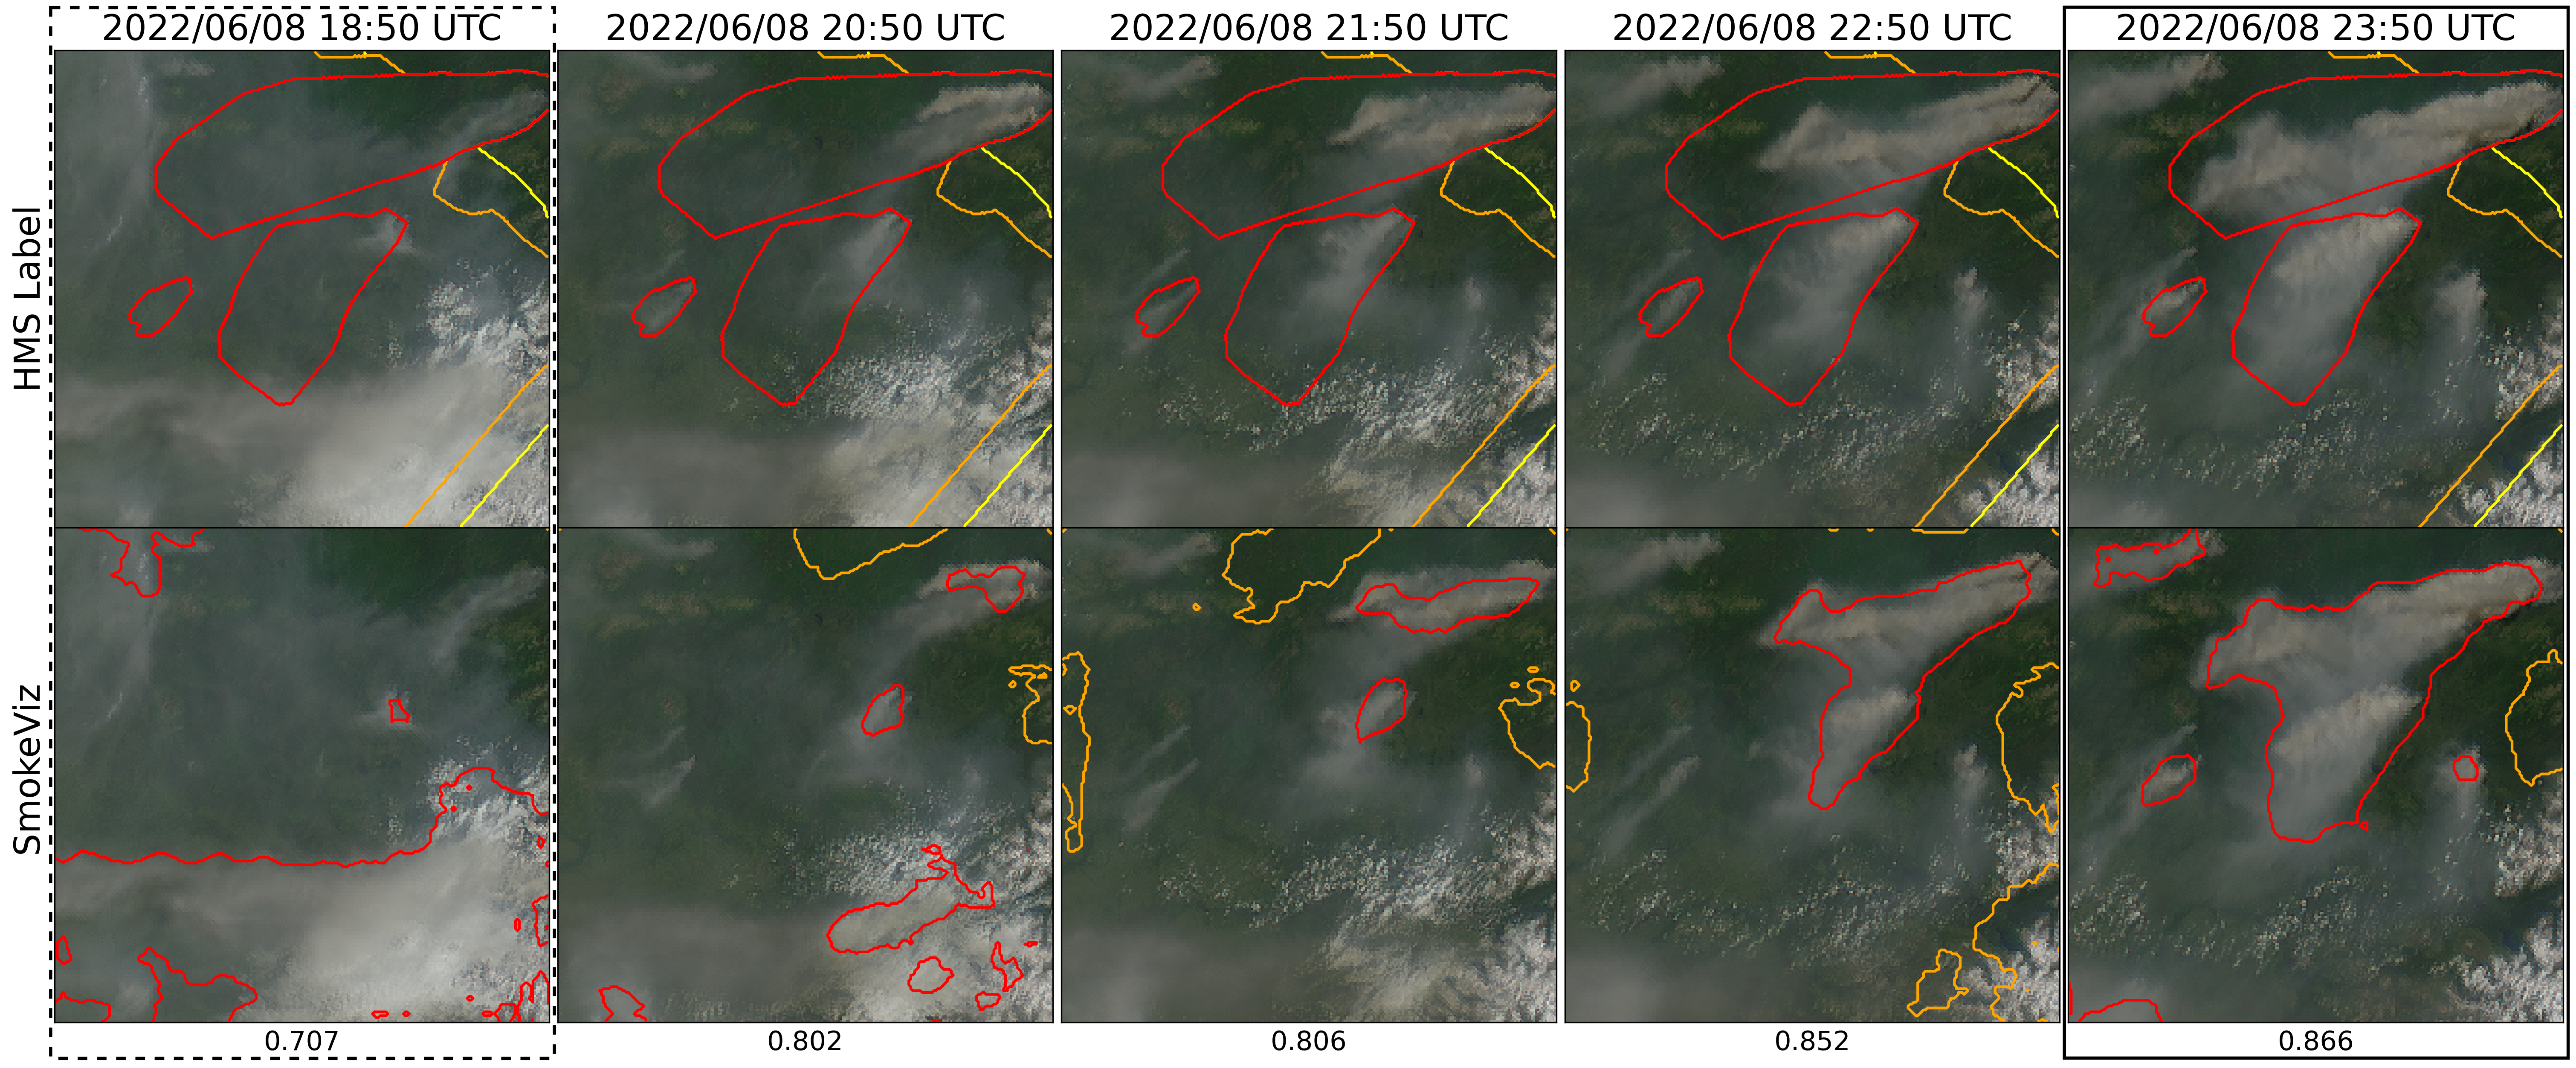
\includegraphics[width=17cm]{figures/final_results.png}
    \caption{GOES-West imagery showing smoke on June 8th, 2022 in Alaska where, at this geolocation (\(61.06^{\circ}\)N, \(156.12^{\circ}\)W), daylight was between 12:43-7:53 UTC. The HMS smoke annotations (top row) span from 18:50 to 23:50 UTC and are compared to the \(f_{\circ}\) generated pseudo-labels (bottom row). The first column (dotted outline) would be the GOES imagery selected for \(\mathcal{X}_{M}\) since it is closest to sunrise. The last column (solid outline) was selected for \(\mathcal{X}_{p}\) since it had the highest IoU value between the pseudo-label and analyst annotation. The IoU score over all densities is reported at the bottom of each column.}
    \label{ml_vs_mei}
\end{figure*}

An illustration of a pseudo-label picked image better representing the analyst annotation when compared to the Mie-derived image selection is evident in Figure \ref{ml_vs_mei}, where the heavy density smoke IoU increases from 0.01 to 0.59. The analyst annotation for these densities cover 5 hours of imagery, the Mie-derived selection optimizes for the image closest to sunrise while the pseudo-label image selection chooses the image with the highest overlap between the pseudo-label and the analyst annotation. The figure also illustrates how using a deep learning model can provide higher time resolution and give a dynamic representation of smoke over time.

To get an idea on how \(f_{c}\) compares to the HMS analyst annotations we show a series of samples from \(\mathcal{X}_{p}\) in figure \ref{bench}. The examples give a qualitative representation of how the predictions from \(f_c\) can provide more detailed boundaries of smoke densities than the HMS annotations do.

\begin{table}[h]
    \caption{Comparison of semantic segmentation model IoU performance on \(\mathcal{X}_{p}\).}\label{bench}
    \centering
    \begin{tabular}{cccrrcrc}
        \toprule
           & DLV3+ & MANet & PSPNet & Linknet \\
        \midrule
        Heavy   & 0.411 & 0.336  & 0.355 & 0.324 \\
        Medium  & 0.484 & 0.487  & 0.502 & 0.456 \\
        Light   & 0.662 & 0.675  & 0.690 & 0.662 \\
        Overall & 0.607 & 0.615  & 0.626 & 0.601 \\
        \bottomrule
    \end{tabular}
\end{table}

The results for the benchmarking models (table \ref{bench}) show similar performance across the models. DeepLabV3+ (\(f_c\)) gives the highest heavy density smoke IoU value, while PSPNet gives the highest overall IoU score.

\begin{figure*}
    \centering
    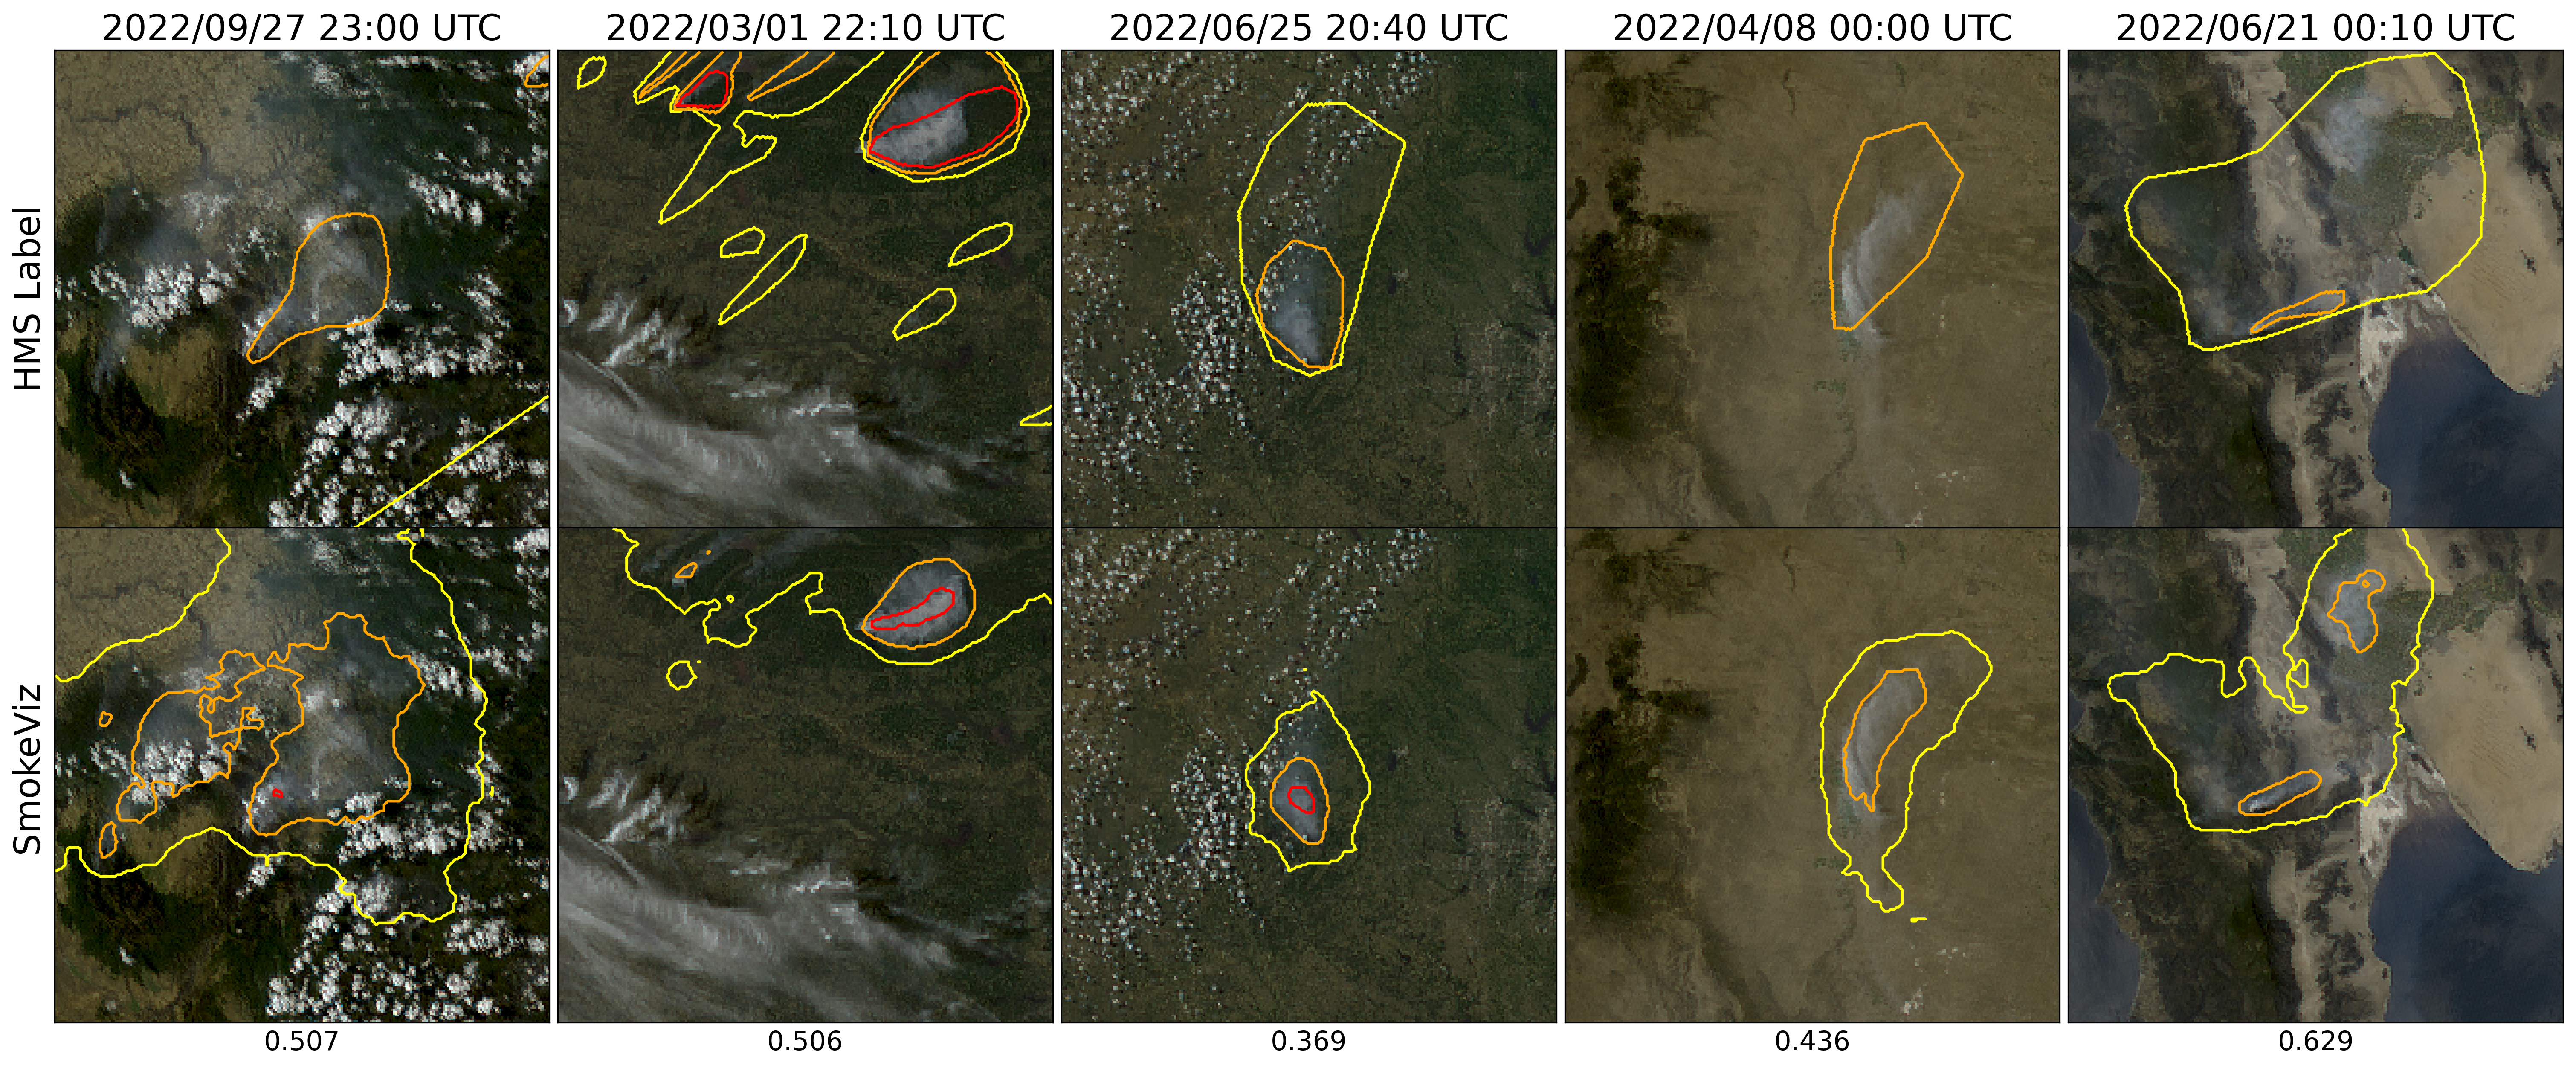
\includegraphics[width=17cm]{figures/examples.png}
    \caption{Examples of HMS annotations (top row) vs \(f_{c}\) output (bottom row) on \(\mathcal{X}_{p}\) samples. The overall IoU score is reported at the bottom of each column.}\label{examples}
\end{figure*}

\section{Limitations}

One of the concerns that comes with using pseudo-labeling methods is that you can perpetuate biases from the parent model into subsequent child models. Due to the increase in detectable forward scattered light off smoke particular matter, we expect the model to have a bias towards producing a higher success rate for smoke detection at larger solar zenith angles. The original HMS annotations do not distinguish by type of fire and include a large representation of controlled agricultural burns. This can be a limitation to consider if the dataset is being trained to target detection of large wildfires. All these limitations are discussed and analyzed further in the Appendix. Additional work should be done to analyze the performance of SmokeViz derived models on dust vs smoke.

\section{Conclusion}

In this study, we have refined an existing dataset originally curated by NOAA's HMS team, transforming it from a many-to-one imagery-to-annotation format to a more succinct, one-to-one satellite image-to-annotation dataset. The initial HMS dataset provided a general approximation of where smoke had been present for a given time window, though it did not guarantee the actual existence of smoke in the labeled pixels during the given times. Our goal was to create a dataset that could be used, along with additional applications, to train a model to detect wildfire smoke in real-time on an image-by-image level. The Mie-derived dataset selection process determined that if smoke was present, what timestamp within the analyst time window would the give the highest smoke signal-to-noise ratio. While optimizing for being able to detect smoke, if it is present, the Mie-dataset selection had no metric to determine if the smoke was effectually present in the selected image. Since many of the images within the HMS time-window either contained no smoke at all or the smoke was not contained within the geospatial bounds of the annotations, the Mie-derived dataset contained a large number of mislabeled samples. Discrepancies between data and labels can be detrimental towards the model's capacity to improve on feature representations in the target domain. During model training, the penalization of accurate predictions can inadvertently introduce biases towards misclassifying noise as meaningful signal. 

To improve the dataset's capacity to accurately represent wildfire smoke plumes, we train a parent machine learning model, \(f_{\circ}\), using the Mie-derived dataset, \(\mathcal{X}_M\), and run it on the relevant satellite images within the time-frame. The image with the maximum IoU score between the model's smoke predictions, or pseudo-label, and the analyst smoke annotations are used to create the pseudo-label generated dataset, \(\mathcal{X}_{p}\). We then train a child model, \(f_c\), using \(\mathcal{X}_{p}\) and test \(f_{\circ}\) and \(f_c\) on both the 2022 testing sets from \(\mathcal{X}_{M}\) and \(\mathcal{X}_{p}\). The results reported in table \ref{iou_results} suggest that \(\mathcal{X}_{p}\) was able to train a better performing model, \(f_c\), that gave higher IoU metrics on both dataset's testing sets in comparison to the original parent model, \(f_{\circ}\).

The result of this study is a representative dataset, SmokeViz, that can be used to train machine learning models for various wildfire smoke applications. A future goal is to produce a robust and reliable machine learning based approach for detecting wildfires using satellite imagery. That information can be used for wildfire detection and monitoring in along with a highly needed smoke product for data assimilation into smoke dispersion models. Additionally, this dataset can be used as a benchmark for how well remote sensing segmentation models can perform on dispersed edges such as smoke. On a broader scale, we show how pseudo-labeling can be used to optimize a dataset when the resolution for the data and corresponding labels do not match. This could be useful in similar applications involving time-series/video data with a singular label where the data can be compressed while still remaining representative of the label. All data is made publically available at [aws download link] and all code can be found at \url{https://github.com/anonymous-smokeviz/SmokeViz}.


{
    \small
    \bibliographystyle{ieeetr}
%    \bibliographystyle{ieeenat_fullname}
    \bibliography{main}
}

% WARNING: do not forget to delete the supplementary pages from your submission 
% \clearpage
\setcounter{page}{1}
\maketitlesupplementary


\section{Rationale}
\label{sec:rationale}
% 
Having the supplementary compiled together with the main paper means that:
% 
\begin{itemize}
\item The supplementary can back-reference sections of the main paper, for example, we can refer to \cref{sec:intro};
\item The main paper can forward reference sub-sections within the supplementary explicitly (e.g. referring to a particular experiment); 
\item When submitted to arXiv, the supplementary will already included at the end of the paper.
\end{itemize}
% 
To split the supplementary pages from the main paper, you can use \href{https://support.apple.com/en-ca/guide/preview/prvw11793/mac#:~:text=Delete%20a%20page%20from%20a,or%20choose%20Edit%20%3E%20Delete).}{Preview (on macOS)}, \href{https://www.adobe.com/acrobat/how-to/delete-pages-from-pdf.html#:~:text=Choose%20%E2%80%9CTools%E2%80%9D%20%3E%20%E2%80%9COrganize,or%20pages%20from%20the%20file.}{Adobe Acrobat} (on all OSs), as well as \href{https://superuser.com/questions/517986/is-it-possible-to-delete-some-pages-of-a-pdf-document}{command line tools}.

\end{document}
